\documentclass[a4paper, 12pt]{report} 

%language and encoding
\usepackage{amsmath}
\usepackage[obeyspaces, spaces]{url}
\usepackage[T1]{fontenc}
\usepackage[utf8]{inputenc}
\usepackage[british,francais]{babel}
\usepackage{parskip}
\usepackage{hyperref}
\usepackage{eurosym}
\usepackage{lmodern}
\usepackage{graphicx}
\usepackage{svg}
\usepackage{pdfpages}
\usepackage{caption}
\usepackage{microtype}
\usepackage{dirtree}
\usepackage{tabto}
\usepackage{rotating}
%police et mise en page (marges) du document	
\usepackage[top=2cm, bottom=2cm, left=3cm, right=3cm]{geometry}
\usepackage{setspace}
\usepackage[nonumberlist]{glossaries}
% C++ style 
\usepackage{listings}
\usepackage{xcolor}
% algorithm
\usepackage[ruled,vlined,french]{algorithm2e}
% colors definition
\definecolor{blue-sii}{RGB}{0,90,163}
\definecolor{purple-sii}{RGB}{141,51,138}
\definecolor{string-color}{RGB}{85, 98, 112}
\definecolor{fun-color}{RGB}{196, 77, 88}
\definecolor{key-color}{RGB}{11, 72, 107}
\definecolor{ponct-color}{RGB}{235,104,65}
\definecolor{comment-color}{RGB}{243, 58, 37}
\definecolor{comment-color}{RGB}{243, 58, 37}
\definecolor{red-stbl}{HTML}{C92525}
% coding style
\lstdefinestyle{customcatkin}
{
  tabsize=4,
  frame=single,
  numbers=left,
  belowcaptionskip=1\baselineskip,
  breaklines=true,
  xleftmargin=\parindent,
  showstringspaces=false,
  language=make,
  commentstyle=\color{comment-color},
  basicstyle={\ttfamily\footnotesize},
  keywordstyle = {\color{key-color}},
  keywordstyle = [2]{\color{comment-color}},
  otherkeywords = {add_definitions, find_package, catkin_package, include_directories, add_executable, target_link_libraries, install,\#},
  morekeywords = [1]{add_definitions, find_package, catkin_package, include_directories, add_executable, target_link_libraries, install},
  morekeywords = [2]{\#},
}
\lstdefinestyle{customcpp}
{
  tabsize=4,
  frame=single,
  numbers=left,
  belowcaptionskip=1\baselineskip,
  breaklines=true,
  xleftmargin=\parindent,
  language=C++,
  showstringspaces=false,
  basicstyle={\ttfamily\footnotesize},
  commentstyle=\color{comment-color},
  %identifierstyle=\color{blue-sii},
  stringstyle=\color{string-color},
  directivestyle=\color{blue},
  keywordstyle = {\color{key-color}},
  keywordstyle = [2]{\color{ponct-color}},
  keywordstyle = [3]{\color{teal}},
  keywordstyle = [4]{\color{string-color}},
  otherkeywords = {;,<<,>>,++,Serializer,nav_msgs,std,cout,endl,serializeMap,append,length,to_string, ||, +, !, =, *,Correlator,feedResult,uint64_t,pair,QObject,WifibotClient,MainWindow,emit,SensorData},
  morekeywords = [1]{emit},
  morekeywords = [2]{;, <<, >>, ++, ||, +, !, =, *},
  morekeywords = [3]{Serializer, nav_msgs, std, serializeMap, cout, endl,to_string,Correlator,feedResult,uint64_t,pair,QObject,WifibotClient,MainWindow,SensorData},
  morekeywords = [4]{append, length},
}
\lstdefinestyle{custombash}
{
  frame=single,
  numbers=left,
  belowcaptionskip=1\baselineskip,
  breaklines=true,
  xleftmargin=\parindent,
  language=bash,
  showstringspaces=false,
  basicstyle={\ttfamily\footnotesize},
  commentstyle=\color{comment-color},
    keywordstyle = [3]{\color{teal}},
  %identifierstyle=\color{blue-sii},
  stringstyle=\color{string-color},
  directivestyle=\color{blue},
  keywordstyle = {\color{key-color}},
  keywordstyle = [2]{\color{key-color}},
  otherkeywords = {roslaunch, float32, Header, string, uint32},
  morekeywords = [1]{float32, Header, string, uint32},
  morekeywords = [2]{roslaunch},
}
\lstdefinestyle{roslaunch}
{
  frame=single,
  numbers=left,
  belowcaptionskip=1\baselineskip,
  breaklines=true,
  xleftmargin=\parindent,
  language=bash,
  showstringspaces=false,
  basicstyle={\ttfamily\footnotesize},
  commentstyle=\color{comment-color},
    keywordstyle = [3]{\color{teal}},
  %identifierstyle=\color{blue-sii},
  stringstyle=\color{string-color},
  directivestyle=\color{blue},
  keywordstyle = {\color{key-color}},
  keywordstyle = [2]{\color{key-color}},
  otherkeywords = {roslaunch},
  morekeywords = [1]{roslaunch}
}
\lstset{escapechar=@}

\makeglossary

\newglossaryentry{SII}
{
  name={SII},
    description={Société pour l'Informatique Industrielle}
}

\newglossaryentry{ROS}
{
  name={ROS},
    description={Robot Operating System}
}

\newglossaryentry{LIDAR}
{
  name={LIDAR},
    description={LIght Detection And Ranging est un dispositif physique muni d'un ou de multiples faisceaux lumineux ainsi que de capteurs permettant la mesure de distances spatiales entre le matériel émetteur et les obstacles rencontrés par les ondes émises}
}

\newglossaryentry{RADAR}
{
  name={RADAR},
    description={RAdar Detection And Ranging}
}

\newglossaryentry{BU}
{
  name={BU},
    description={Une Business Unit est une unité organisationnelle au sein d'une entreprise, s'articulant autour d'un domaine d'activité donné. Par la création de BU, 
    l'entreprise entend généralement augmenter son chiffre d'affaires et sa marge brute en conférant 
    d'avantage d'autonomie financière et décisionnelle à ces unités stratégiques. On parle également de département, de division ou de domaine fonctionnel}
}

\newglossaryentry{ASD}
{
  name={ASD},
    description={Aero Space Defense est une Business Unit définie par SII}
}

\newglossaryentry{SA}
{
  name={SA \`{a} directoire et conseil de surveillance},
    description={Une Société Anonyme est une forme juridique de société commerciale, dont la dénomination sociale permet entre-autre de protéger l'anonymat de ses actionnaires. 
    SII correspond à une SA à directoire et conseil surveillance.
    Moins répandue qu'une SA à conseil d'administration\cite{Bib_SA_wiki}, ce statut mène à identifier distinctement deux organes de gouvernance dont le directoire représente la partie exécutive. 
    Le conseil de surveillance endosse quant à lui les tâches de nomination et de contrôle du directoire}
}

\newglossaryentry{NTIC}
{
  name={NTIC},
    description={Nouvelles Technologies de L'Information et de la Communication}
}

\newglossaryentry{SI}
{
  name={SI},
    description={Système d'Information}
}

\newglossaryentry{IDF}
{
  name={IDF},
    description={\^{I}le-de-France}
}

\newglossaryentry{ETR}
{
  name={ETR},
    description={Energie Transport Retail est une Business Unit définie par SII}
}

\newglossaryentry{BAM}
{
  name={BAM},
    description={Banque Assurance Mutuelle est une Business Unit définie par SII}
}

\newglossaryentry{POC}
{
  name={POC},
    description={Proof Of Concept (preuve de concept)}
}

\newglossaryentry{QHSE}
{
  name={QHSE},
    description={Qualité Hygiène Sécurité Environnement. Située au niveau de l'agence \^{I}le-de-France, la cellule QHSE veille activement sur le respect de la qualité opérationnelle, tout en s'inscrivant dans une démarche d'amélioration continue. 
    Elle est en charge de la préparation et du maintien des niveaux de certifications de l'entreprise.
    Enfin, elle est impliquée dans la mise en pratique d'une démarche \gls{RSE}, notamment par la prise en compte des impacts environnementaux de l'activité}
}

\newglossaryentry{RSE}
{
  name={RSE},
    description={Responsabilité Sociétale de l'Entreprise}
}

\newglossaryentry{RD}
{
  name={R\&D},
    description={Recherche et Développement}
}

\newglossaryentry{SRT2M}
{
  name={SRT2M},
    description={Système Robotique Tactique Multi-Missions pour la surveillance et l'aide à la prise de décisions dans les milieux à risques. 
    C'est le nom donné au système final intégrant les briques logicielles et physiques issues de mon stage et de celui de M. Chazot}
}

\newglossaryentry{DCL}
{
  name={DCL},
    description={Document de Conception du Logiciel}
}

\newglossaryentry{STBL}
{
  name={STBL},
    description={La Spécification Technique du Besoin Logiciel est un document généralement réalisé par un client pour spécifier le besoin qui justifie la réalisation d'un logiciel}
}

\newglossaryentry{SDK}
{
  name={SDK},
    description={Software Development Kit}
}

\newglossaryentry{IHM}
{
  name={IHM},
    description={Interface Homme-Machine}
}

\newglossaryentry{classe}
{
  name={classe},
    description={La classe d'un objet correspond à un champ textuel qui permet de le qualifier. Ce label est fourni par le réseau neuronal et résulte des opérations de détection et de classification.
    Par exemple, on peut observer les classes "humain", "chaise" ou "ordinateur" pour un réseau neuronal destiné à être employé dans un environnement de bureau}
}

\newglossaryentry{landmarks}
{
  name={points de repères},
    description={Les points de repère sont des caractéristiques observables par le biais de capteurs du robot, lui permettant de se situer dans son environnement et de le carographier. 
    La qualité d'un point de repère s'évalue en fonction des caractéristiques suivantes :
    \begin{itemize}
    \item la facilité de ré-observabilité
    \item la possibilité de discrimines des poinst de repères individuels 
    \item leur quantité dans l'environnement
    \item leur caractère stationnaire
    \end{itemize}
    Un exemple typique est une ligne droite et des coins bien définis tels que des murs délimitant une pièce}
}

\newglossaryentry{KNN}
{
  name={KNN},
    description={K-Nearest Neighbor est un algorithme qui permet de définir la sortie associée à une entrée donnée en considérant les K plus proches voisins connus de cette entrée. 
    La notion de voisinnage est sous-tendue par l'application d'une formule de distance entre l'entrée à traiter et les échantillons connus}
}

\newglossaryentry{XMLRPC}
{
  name={XML-RPC},
    description={XML-RPC est un protocole réseau de type \emph{Remote Procedure Call} permettant l'échange de données et l'appel de méthodes par des exécutables distincts. La définition des données 
    comme des procédures est faite par le biais du langage XML}
}

\newglossaryentry{topics}
{
  name={topics},
    description={Les topics permettent la communication entre les différents noeuds. 
    Un noeud est responsable de la publication des données du topic (commandes de contrôle par exemple) et un noeud distinct souscrit à ce même topic pour les récupérer (par exemple le noeud qui va traîter ses commandes).
    Typiquement, la publication d'un topic se fera en C++ par l'appel à la méthode advertise().
    Parallèlement, la souscription a un topic nécessite l'appel à la méthode subscribe()}
}

\newglossaryentry{services}
{
  name={services},
    description={Les services sont des éléments de communication inter-noeuds qui permettent l'envoi de requêtes et de réponses. 
    La création de services passe par la définition textuelle des types de données attendues dans la requête et la réponse}
}

\newglossaryentry{serveur de parametres}
{
  name={serveur de paramètres},
    description={Le serveur de paramètres est un dictonnaire partagé entre les différents noeuds actifs, accessible grâce aux APIs réseaux. 
    Il n'est pas destiné à supporter une montée en charge importante, de telle sorte que son utilisation doit se limiter à stocker les paramètres d'utilisation des noeuds. 
    Ces derniers pourront récupérer leurs variables de configuration au runtime en invoquant le serveur.
    Le serveur de paramètre utilise le protocole XMLRPC et est impélmenté à l'intérieur du ROS Master}
}

\newglossaryentry{Catkin}
{
  name={Catkin},
    description={Catkin est le nom de la chaîne de compilation utilisée par ROS. 
    Basée sur des macros CMake, catkin automatise un certain nombre de tâches, dont la recherche de packages ROS. 
    Ainsi, Catkin permet la génération d'exécutables, de librairies, d'interfaces exportées ou de scripts auto-générés, 
    chacune de ces cibles devant apartenir et être générées depuis un package contenant le code source requis}
}

\newglossaryentry{SLAM}
{
  name={SLAM},
    description={Le SLAM pour Cartographie et Localisation Simultannées (de l'anglais Simultaneous Localisation And Mapping) est une discipline permettant 
    de conférer à un dispositif mobile la perception de son environnement externe, sous la forme d'une cartographie des points de repères stationnaires, tout comme de ses 
    propres positions et orientations au sein de cet environnement. 
    Le SLAM est mis en \oe{}uvre par le biais de capteurs internes (mesures odométriques ou inertielles) et externes (LIDAR, RADAR, caméra)}
}

\newglossaryentry{Hector SLAM}
{
  name={Hector SLAM},
    description={Hector SLAM est le nom d'un métapackage ROS disponible par le biais du gestionnaire de version Git. 
    Il contient entre-autres un n\oe{}ud de SLAM, nommé hector\_mapping. Hector SLAM est sous licence BSD et a été développé par des chercheurs de l'université de Darmstad (Allemagne) dont 
    Stefan Kohlbrecher et Johannes Meyer. Ses fondements théoriques apparaissent dans une publication datant de 2011\cite{Bib_Hector_SLAM}}
}

\newglossaryentry{IMU}
{
  name={IMU},
    description={Inertial Measurement Unit, désigne des données issues de capteurs inertiels, typiquement présents dans des systèmes robotiques ou des véhicules aériens sous la forme de gyromètres et d'accéléromètres.
    De telles mesures qualifient le roll, le pitch et le yaw (roulis, tangage et lacet en français), à savoir les valeurs des composantes sur les trois degrés de liberté d'un véhicule }
}

\newglossaryentry{GeoTIFF}
{
  name={GeoTIFF},
    description={Tf pour ``The transform library'' est un package ROS qui permet de mettre en relation différents systèmes de coordonnées et de mettre à jour ces relations durant leurs déplacements respectifs}
}

\newglossaryentry{bagfile}
{
  name={bagfile},
    description={Un fichier bag (ou bagfile) est un fichier spécifique à l'écosystème de ROS qui contient des enregistrements de messages sérialisés variés et les timestamps afférents. 
    ROS permet l'enregistrement et la lecture de tels fichiers par le biais d'outils tels que l'exécutable rosbag.
    Ces fichiers sont utilisés à des fins d'analyse ou de simulations de situations pratiques pendant lesquelles des n\oe{}uds émettent et / ou transmettent des données}
}

\newglossaryentry{tf}
{
  name={tf},
    description={Tf, pour \emph{The transform library} est le nom d'un package ROS qui permet de définir les nomenclatures et les transformations entre les systèmes de repères utiles aux n\oe{}uds de calcul}
}

\newglossaryentry{TCP}
{
  name={TCP},
    description={Transport Control Protocol est un protocole de la couche transport qui permet entre-autre la remise d'accusés de réception à l'émetteur (flag ACK) dans un environnement client-serveur. 
    Cette particularité vise à assurer la fiabilité de la communication établie}
}

\newglossaryentry{EKF}
{
  name={EKF},
    description={Extended Kalman Filter}
}

\newglossaryentry{API}
{
  name={API},
    description={Application Programming Interface est une interface donnant accès à un ensemble de méthodes et fonctions normalisées facilitant le développement d'applications}
}

\newglossaryentry{XML}
{
  name={XML},
    description={eXtensible Markup Language est un langage informatique balisé et normalisé, traditionnellement utilisé à des fins de transmission de données via Internet de part son indépendance de toute plateforme}
}

\newglossaryentry{Kanban}
{
  name={Kanban},
    description={Mot japonais signifiant  ``étiquette''. 0ans le domaine du développement logiciel le Kanban (issu de la méthode japonaise du même nom) consiste à instaurer des métriques visuelles attestant l'avancement d'un projet tout en facilitant sa gestion. 
    Il s'agit généralement d'un tableau où chaque colonne correspond à une étape du processus de réalisation et au travers duquel on déplace des items de gauche vers la droite en fonction de l'état dans lequel ils se trouvent}
}

\newglossaryentry{SCRUM}
{
  name={SCRUM},
    description={SCRUM est une méthode AGILE apparue au début des années 1990, basée sur l'empirisme et l'amélioration continue. Les principes clés sont aujourd'hui exposés dans un document de référence appelé SCRUM guide}
}

\newglossaryentry{USAR}
{
  name={USAR},
    description={Urban Search And Rescue, est un terme qui qualifie les environnements, scénarios ou situations impliquant la recherche, la mise à l'abri et parfois les soins de victimes en espace urbain. 
    Un exemple typique consiste à évacuer des victimes d'un immeuble incendié}
}

\begin{document}

  \pagestyle{empty}
  %%%%%%%%%%%%%%%%%%%%%%%%%%%%%%%%%%%%%%%%%%%%%%%%%%%%%
  %                    Blank                          %
  %%%%%%%%%%%%%%%%%%%%%%%%%%%%%%%%%%%%%%%%%%%%%%%%%%%%%
 
  \newpage
  ~ 
  \newpage
  
  %%%%%%%%%%%%%%%%%%%%%%%%%%%%%%%%%%%%%%%%%%%%%%%%%%%%%
  %                    Abstract                       %
  %%%%%%%%%%%%%%%%%%%%%%%%%%%%%%%%%%%%%%%%%%%%%%%%%%%%%
  
  \newpage
  \begin{abstract}
    Pour répondre aux besoins qui motivent leur réalisation, les systèmes robotiques mobiles doivent s'appuyer sur une connaissance plus ou moins fiable de leur environnement. 
    On distingue la perception de l'environnement externe du robot de la perception que le robot a de lui-même --en tant que plateforme mobile-- au sein de cet environnement.
    Ces deux versants, qui tiennent une place prépondérante dans le domaine des véhicules autonomes ou intelligents, 
    sont connus sous le nom de SLAM (Localisation et Cartographie Simultannées). 
    Ce rapport aborde ces questions au travers de la spécification, de la conception et de l'implémentation de briques logicielles destinées à contrôler un robot mobile 
    et rendre état de son environnement externe tout comme de sa localisation en temps réel.   
    Le projet décrit dans ce document recouvre le système complet, allant des périphériques physiques d'acquisition de données jusqu'à la présentation des résultats au travers d'une 
    IHM interactive. 

    In order to carry out specific tasks, robotic systems must rely on a consitent environment perception. 
    Two types of environment perception can be distinguish. The first is about external environment, and the second is about the location of the mobile plateform in this environment.   
    These two complementary aspects are known as SLAM (Simultaneous Localisation And Mapping). 
    This report adresses these issues through the specificaiton, the conception and the implementation of software components. 

  \begin{center}
    \textbf{Mots-clés}
    
    Cartographie et Localisation Simultannées
    
    Développement logiciel
    
    Temps-réel
    
    Système embarqué
    
    Robot Operating System
  
  \end{center}
\end{abstract}

  %%%%%%%%%%%%%%%%%%%%%%%%%%%%%%%%%%%%%%%%%%%%%%%%%%%%%
  %                  ThanksGiving	              %
  %%%%%%%%%%%%%%%%%%%%%%%%%%%%%%%%%%%%%%%%%%%%%%%%%%%%%

  \chapter*{Remerciements}

En prélude à ce rapport, je tiens à remercier M. David Daumand, ingénieur logiciel au sein de la société \gls{SII}, qui a défini, tutoré et défendu ce projet. 
Merci à lui pour le suivi et l'implication sans faille sur lesquels j'ai pu compter durant ces six mois, et ce malgré les efforts organisationnels qui lui incombaient.
J'ai tout particulièrement apprécié la passion pour les sujets de robotique et de développement qu'il a su transmettre avec patience et surtout, avec un enthousiasme constant.
Ce stage se concluant par une embauche, je ne pourrais que souligner la part importante qu'il a jouée dans le cheminement menant à cette situation et les conseils expérimentés qu'il a pu prodiguer à cet effet. 

Je salue sincèrement M. Adel Hafiane, enseignant-chercheur et responsable du laboratoire de vision par ordinateur de l'INSA Centre Val-de-Loire, qui m'a assistée en qualité d'enseignant-référent.
Je le remercie d'avoir veillé assidûment sur ce projet, tant dans les conditions matérielles de son déroulement, que dans son orientation technique et pédagogique au regard de ma formation. 
J'exprime toute ma gratitude à son égard pour nous avoir, Alban Chazot et moi, orientés vers \gls{SII} pour nos stages de fin d'étude avec la confiance qui était la sienne. 

Enfin je remercie l'ensemble de l'équipe qui m'a accueillie avec bienveillance, sympathie et humanité au sein de l'agence de \gls{SII} Bourges. 
Merci aux consultants, stagiaires, Responsable de site et collaborateurs 
qui ont jalonné mon quotidien et enrichi mon expérience professionnelle nouvelle dans ses aspects techniques, organisationnels et bien sûr humains. 
  \thispagestyle{empty}
  %%%%%%%%%%%%%%%%%%%%%%%%%%%%%%%%%%%%%%%%%%%%%%%%%%%%%
  % 	           Table of Contents                  %
  %%%%%%%%%%%%%%%%%%%%%%%%%%%%%%%%%%%%%%%%%%%%%%%%%%%%%
  
  \pagebreak
  
  \tableofcontents
  
  \pagebreak
  
  %%%%%%%%%%%%%%%%%%%%%%%%%%%%%%%%%%%%%%%%%%%%%%%%%%%%%
  %                  Figures & Tabs		      %
  %%%%%%%%%%%%%%%%%%%%%%%%%%%%%%%%%%%%%%%%%%%%%%%%%%%%%
  
  \listoffigures
  
  %%%%%%%%%%%%%%%%%%%%%%%%%%%%%%%%%%%%%%%%%%%%%%%%%%%%%
  % 	                Chapters                      %
  %%%%%%%%%%%%%%%%%%%%%%%%%%%%%%%%%%%%%%%%%%%%%%%%%%%%%
 
  \chapter*{Introduction}
\addcontentsline{toc}{chapter}{Introduction}

\addtocontents{toc}{\protect\thispagestyle{empty}}
\addtocontents{lof}{\protect\thispagestyle{empty}}

Issu d’un partenariat entre \gls{SII} et l’INSA Centre Val-de-Loire, ce stage vise à la réalisation d’une application logicielle au sein de la société SII, sur le site de Bourges. 
Il s’inscrit dans le domaine du développement informatique appliqué à la robotique. 
Les briques logicielles implémentées devront permettre de contrôler un robot mobile, de cartographier son environnement, ainsi que de le localiser en temps réel au travers d'une \gls{IHM} interactive. 
Les versants de cartographie et de localisation sont également connus sous le terme de \gls{SLAM} pour cartographie et localisation simultanées. 
Ils s’appuient en priorité sur des mesures spatiales, fournies par un \gls{LIDAR} embarqué sur le robot et --dans une moindre mesure-- sur les relevés d'encodeurs présents au niveau des roues du robot.
Au travers de sa mise en \oe{}uvre, le \gls{SLAM} constitue une base indispensable à tout système de navigation autonome. 
Bien que ce point ne fasse pas l'objet de ce rapport, il constitue en grande partie l'essence applicative du présent projet. 

Les réalisations attendues s'inscrivent en effet dans un périmètre plus large qu’est la mise en \oe{}uvre d’un Système Robotique Tactique Multi-Missions pour la surveillance et l’aide à la prise de décisions dans les milieux à risques (\gls{SRT2M}).
Adressé au secteur de la Défense, ce système en devenir permet à un opérateur humain d’effectuer des missions de contrôle, de surveillance et de recherche en terrain dangereux ou potentiellement dangereux directement depuis un ``shelter'', à savoir une zone abritée. 
L’opérateur dispose à cet effet d’une flotte de robots terrestres et aériens qu’il contrôle à distance. 
L'exploration du milieu permet d'une part la visualisation de données cartographiques et la localisation des véhicules au sein de la carte, et d’autre part, la réception
de flux vidéo émanant de caméras à 360\degre embarquées. 
Ces flux vidéo sont soumis à des traitements qui permettent de détecter des objets d’intérêt et de les classifier de manière automatique. 
C'est Alban Chazot, également étudiant ingénieur à l'INSA Centre Val-de-Loire, qui a assuré la réalisation de cette dernière fonctionnalité.   
Les classifications sont ensuite incrustées sur la carte générée, de manière à ce que l'utilisateur puisse visionner les résultats de \gls{SLAM}, la \gls{classe}, la position et la taille des entités détectées en une seule et même zone de rendu. 

Le premier chapitre vise à apporter au lecteur une compréhension suffisante du contexte du stage pour en saisir les enjeux. 
Il s'attache d'abord à décrire la structure d'accueil, à savoir le groupe \gls{SII}, au sein duquel s'articulent les agences françaises et en particulier, l'agence \^{I}le-de-France
dont dépend le site de Bourges. 
\`{A} ce titre, sa portée et son organisation seront particulièrement détaillées. \\
Un deuxième chapitre donnera les étapes les plus conséquentes de la réalisation. 
Cette restitution consistera d'abord à définir clairement le livrable attendu à la fin du stage notamment au travers de l'analyse fonctionnelle du produit.
Une partie viendra étayer les choix techniques ou théoriques qui constituent la base de l'implémentation, comme les principes fondamentaux du \gls{SLAM} ou l'utilisation de \gls{ROS}. 
Puis nous discuterons la façon dont ces principes ont été intégrés au projet, au travers d'éléments qui relèvent de la mise en \oe{}uvre architecturale et du fonctionnement général de l'application résultante.\\
Ce document sera complété d'un chapitre destiné à exposer les stratégies organisationnelles mises en place durant les différentes phases d'avancement du stage. 
Nous décrirons également les résultats obtenus et les suites envisagées pour le projet, ainsi que les perspectives individuelles au sein de la structure d'accueil. \\
Enfin, ce rapport s'accompagne d'un glossaire visant à détailler les acronymes, termes techniques ou peu communs que le lecteur est susceptible de rencontrer. 
  \pagestyle{plain}
  \setcounter{page}{1}
  \chapter{L'environnement du stage, la Société pour l'Informatique Industrielle}

\section {Introduction}
Ce chapitre vise à apporter au lecteur une compréhension suffisante du contexte du stage pour en saisir les enjeux. 

Il s'attache d'abord à décrire la structure d'accueil, à savoir le groupe \gls{SII}, au sein duquel s'articulent les agences françaises et en particulier, l'agence \^{I}le-de-France.
Cette dernière englobe la structure berruyère qui a hébergé le stage. \`{A} ce titre, sa portée et son organisation seront particulièrement détaillées. 

Nous spécifierons ensuite les axes stratégiques qui justifient la mise en oeuvre du projet. 
Une section décrira l'apport souhaité du projet pour SII tandis que la section suivante reviendra sur un acteur particulier de l'écosystème de l'entreprise : l'INSA Centre Val-de-Loire, qui s'inscrit en partenaire financier, 
stratégique et organisationnel en amont de ce projet.

\section{Principaux repères et évolution de la structure SII}

\subsection{Signalétique générale : du groupe à l'agence parisienne}

Couramment nommée \gls{SII}, la Société pour l'Informatique Industrielle est une \gls{SA}, aujourd'hui implantée dans dix-huit pays, sur quatre continents.

Sur l'exercice 2015/2016, le groupe SII enregistre un chiffre d'affaires consolidé de 360,1M\euro\cite{Bib_exercice_2015_2016}, pour un résultat net de 13.13M\euro\cite{Bib_exercice_2015_2016}, et compte sur un effectif moyen de 5 226 collaborateurs\cite{Bib_exercice_2015_2016}. 

Depuis plus de 30 ans\cite{Bib_exercice_2015_2016}\cite{Bib_memento_ag_idf}, SII \oe{}uvre pour s'inscrire en tant que partenaire technologique de choix auprès d'une clientèle professionnelle diversifiée. 
Le groupe --qui a consolidé son expérience dans quatorze secteurs d'activités disctincts-- propose des offres liées aux savoir-faire suivants : 

\begin{itemize}
 \item \textbf{L'informatique embarquée} incluant le développement de logiciels embarqués, de contrôle commande ou encore de bancs de tests   
 \item \textbf{L'ingénierie scientifique} qui balaye les champs de l'électronique, du traitement du signal et de la mécanique
 \item \textbf{Les \gls{NTIC}}, englobant les problématiques de téléphonie, de web, de mobilité ou d'infrastructures diverses
 \item \textbf{Les Systèmes d'Informations} qui recouvrent l'informatique décisionnelle, financière ou la sécurité du \gls{SI}
\end{itemize}

Les secteurs d'activités s'organisent quant à eux en \gls{BU}. Chacune de ces unités s'adresse à un groupe de clients majeurs et détient un organigramme interne, placé sous la responsabilité du Directeur de \gls{BU}. 

L'agence Île-de-France est une des neuf agences françaises de la société. Elle est placée sous la responsabilité du Directeur d'Agence, M. Didier Bonnet.
Son administration est abritée sur le site de Kennedy\footnote{104 Avenue du Président Kennedy, 75016 Paris} --principalement dédié aux opérations de gestions-- et recouvre deux sites supplémentaires : celui du 
Dynasteur\footnote{6, 12, 10 Rue Andras Beck, 92360 Meudon} et celui de Bourges\footnote{14, allée Charles Pathé, 18000 Bourges } au sein duquel s'est déroulé ce stage. 

Les activités de réalisations se concentrent pour cette agence autour de quatre secteurs d'activités qui sont présentés figure \ref{fig:BU-IDF}. 

\begin{figure}[h]
  \centering
    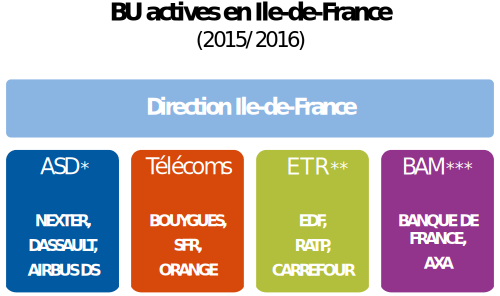
\includegraphics[width=.5\linewidth]{figures/BU-clients-IDF}
    \caption*{*Aero-Space Defense, **Energie Transport Retail, ***Banque Assurance Mutuelle}  
  \captionof{figure}{BU actives en IDF}
  \label{fig:BU-IDF}
\end{figure}

Pour ces secteurs, un portefeuille de dix clients est responsable de 80\% du chiffre d'affaires annuel de l'agence. 
La figure \ref{fig:BU-IDF} donne la nomenclature des \gls{BU} définies par l'entreprise, et illustre la clientèle française qui leur est associée.  

\subsection{\'{E}volution de SII en France et à Bourges}

SII a été créée à Paris en 1979 par un ingénieur, Bernard Huvé, qui en est aujourd'hui le Président du Conseil de Surveillance. 
S'en suivra la création de multiples agences provinciales, jusqu'en 1999 où, forte de 400 collaborateurs et d'une croissance soutenue, la société s'introduit en bourse.  
On peut relever l'internationalisation de SII, qui intervient en 2006 avec l'ouverture d'une filiale en Pologne, pour atteindre aujourd'hui un total de 17 filiales à l'étranger\cite{Bib_exercice_2015_2016}.  

Dans ce qui va suivre, nous nous concentrons uniquement sur l'implantation française de SII, qui se retrouve à présent au travers 22 sites sur le territoire.  

\begin{figure}[h]
    \centering
    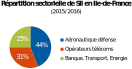
\includegraphics[width=.5\linewidth]{figures/BU-IDF}
    \captionof{figure}{Répartition sectorielle de SII en IDF\cite{Bib_memento_ag_idf}}
    \label{fig:Rep-sectorielle}
\end{figure}

Aujourd'hui, les secteurs d'activités clés de l'entreprise peuvent être classés selon deux catégories\cite{Bib_memento_ag_idf}, que la figure \ref{fig:Rep-sectorielle} permet de justifier : 

\begin{itemize}
  \item \textbf{Les secteurs stratégiques}, que sont \gls{ASD} et Télécoms. Etant des générateurs forts de valeur, ils concernent des marchés mûrs où SII a su établir des relations pérennes avec ses clients grand-compte. 
  \item \textbf{Les secteurs de conquête}, inclus dans les \gls{BU} \gls{ETR} et \gls{BAM}, amenés à se digitaliser massivement
\end{itemize}

Dirigée par M. Fabrice Bosch, l'agence berruyère compte quant à elle une cinquantaine de collaborateurs répartis sur les secteurs d'activités \gls{ETR} et \gls{ASD}. 
Elle héberge également des activités de \gls{QHSE} sous la responsabilité de M. Jean-Sébastien Salis.  

Les activités \gls{ETR} se concentrent sur le développement de solutions billetiques pour des acteurs majeurs du transport de voyageurs. 
En parallèle, les activités \gls{ASD} sont tournées vers un ensemble d'acteurs du secteur de l'armement et de la Défense historiquement implantés à Bourges et, aujourd'hui encore, essentiels à l'économie locale\cite{Bib_def_cher}. 
Parmi ces clients ont peut citer la filiale missilière du groupe Airbus MBDA, ou encore Nexter Munitions dont le site de Bourges accueille les ingénieurs et cadres affilés aux missions de \gls{RD} . 
Enfin, et au regard du caractère critique des missions relevant de la défense nationale ou européenne, on notera que le site de Bourges dispose d'une habilitation à mener au sein de son infrastructure des projets classés Confidentiel
Defense. 

\section{Une mission R\&D pour b\^{a}tir de nouvelles offres}

\subsection{SII Research dans l'agence berruyère}

La mission qui m'a été confiée durant ce stage est placée sous l'égide de l'entité SII Research. 
Sous la responsabilité du Pôle Innovation, cette structure permet de mener à bien des projets transverses aux différents secteurs d'activités, financés sur les fonds propres de l'entreprise.  

Typiquement, ce type de projet sera qualifié de \gls{POC} ou démonstrateur. Pour l'entreprise d'accueil, les réalisations sont menées avec les objectifs suivants : 

\begin{itemize}
  \item Valoriser l'expertise de l'entreprise dans des domaines techniques précis et actuels
  \item Elargir les connaissances internes en communiquant autour des savoir-faire sollicités
  \item Bâtir de nouvelles offres à partir de tout ou partie du \gls{POC} 
\end{itemize}

Ces réalisations permettent de communiquer techniquement avec des acteurs internes et des parties prenantes externes (clients, prospects ou étudiants) --notamment par le biais de médias sociaux-- sans compromettre la confidentialité 
de projets clients. 

Ce projet s’inscrit dans la mise en \oe{}uvre d’un Système Robotique Tactique Multi Missions pour le Surveillance et l’Aide à la Prise de Décisions dans les Milieux à Risques, adressé au secteur de la Défense 
et, plus particulièrement, aux clients berruyers de la \gls{BU} \gls{ASD}.
Dans cette optique, le stage s'est d'emblée accompagné de l'objectif ambitieux d'être véhiculé auprès de représentants de l'entreprise Nexter Systems, à son terme ou durant des stages suivants.  
Ainsi, plusieurs jalons ont pu être posés avec succès dans le respect des procédures internes de validations hiérarchiques. 
Il a notamment pu être présenté à MM. Giraud-Sauveur et Boucher respectivement commercial / chargé d'affaires sur le périmètre MBDA / Nexter et Directeur de projets Nexter. 
Accompagné d'une démonstration, cet entretient s'est soldé positivement et a permis au \gls{POC} d'être relayé par la suite aurpès des instances susceptibles d'assurer son pilotage futur.  

\subsection{Fruits du partenariat avec l'INSA Centre Val-de-Loire}

Ce stage --comme celui d'Alban Chazot-- s'effectue dans le cadre d'un partenariat entre SII et l'INSA Centre Val-de-Loire. 
La relation établie entre ces deux entités découle de la convention ``Carré des partenaires'' acceptée par les deux parties en 2015.
Quentin Ménart, aujourd'hui ingénieur logiciel au sein de l'agence SII Bourges nous a précédés en expérimentant l'année dernière un stage découlant du partenariat.  

Cette relation privilégiée mène à retrouver SII en qualité d'acteur ou de sponsor de certains évènements majeurs de la vie étudiante : Nuit de l'Info, Forum des entreprises, conférences techniques.
Par ailleurs, elle permet de favoriser l'accueil de stagiaires et d'alternants en provenance de l'institut.  

\begin{figure}[h]
    \centering
    \includegraphics[width=.4\linewidth]{figures/wifibot}
    \captionof{figure}{Wifibot embarquant un RPLidarA2 et une caméra Theta S}
    \label{fig:Wifibot}
\end{figure}

En ce qui nous concerne, cette collaboration a impacté nos stages de manière visible et fructueuse.
En effet, elle a permis le prêt d'un robot mobile par M. Benali Abderraouf, enseignant-chercheur en robotique à l'INSA Centre Val-de-Loire. 
Ce robot qui a constitué la base du projet est présenté sur la figure \ref{fig:Wifibot}.
Dans ce cadre, l'INSA Centre Val-de-Loire a également financé pour moitié le matériel nécessaire au projet, à savoir une caméra Theta S à 360\degre (cf. figure \ref{fig:Wifibot}).

Ce partenariat a aussi donné lieu à des réunions régulières de co-pilotage de projet réunissant MM. Hafiane et Bosch. 
Elles nous ont permis de réfléchir ensemble au cap à donner, au matériel à acquérir ou encore aux techniques à employer.
Enfin, nous avons pu évoluer sereinement en qualité de stagiaires, en comptant sur le suivi fréquent de M. Adel Hafiane, tant dans la mise en place du projet, que durant les phases plus tardives de développement.

  \chapter{Définition et mise en oeuvre d'un système de SLAM en temps-réel}

\section{De l'expression du besoin à une spécification complète}

  \subsection{Vision et cas d'utilisation}

Les réalisations effectuées ont été guidées par une phase d'analyse du besoin, menée de concert avec les membres de l'équipe projet. 
En qualité de tuteur de stage, M. David Daumand a guidé ce projet afin que le système final implique des perspectives commerciales concrètes. 
Dans cette optique, il a apporté son expertise sur ce que seraient les besoins de clients potentiels, en orientant la démarche vers une application militaire. 
Il a ainsi défini la dénomination du système \gls{SRT2M}, permettant à elle seule d'exprimer la fonction, le contexte et le secteur visé par le produit.  

La preuve de concept réalisée durant ce stage est un sous-système de \gls{SRT2M}. 
Afin d'en exposer clairement le périmètre, la figure \ref{fig:use-case} défini sa nomenclature et en donne les principaux cas d'utilisation. 

\begin{figure}[h]
  \centering
    \includegraphics[width=.8\linewidth]{figures/use-case-test}  
  \captionof{figure}{Diagramme de cas d'utilisation du système de cartographie et de localisation d'un robot mobile}
  \label{fig:use-case}
\end{figure}

Ainsi, ce \emph{sous-système} doit permettre d'effectuer une cartographie de l'environnement d'un robot mobile, tout en donnant sa localisation. 
L'acteur primaire du système pourra visualiser une carte, soit à partir de données préalablement sauvegardées au sein de ce même système, soit grâce à des données acquises en temps réel par des périphériques dédiés. 
Cette visualisation implique la représentation d'obstacles statiques dans l'espace exploré, mais aussi la position et la trajectoire du robot en tout temps.
Le téléguidage du robot par l'utilisateur doit également être assuré. 
Un opérateur --typiquement un contributeur du système-- pourra jouer sur les paramètres de présentation des résultats, de la mise en réseau des périphériques ou de la définition de ces périphériques. 

Divers périphériques sont à ce stade réunis en un seul acteur ``Périphérique matériel''.
Il inclut le \gls{LIDAR} et le robot qui permettent respectivement d'acquérir les mesures de distances aux obstacles et de déplacer la plateforme.
On souligne aussi la présence d'un ``Composant logiciel'' qui interagit avec le système.
Ce composant est vu comme une boîte noire qui fournit en sortie les résultats de détection et de classification d'objets d'intérêt rencontrés par le système.
Dans les faits, ces résultats correspondent à la position, la taille et la \gls{classe} de chaque objet, ce qui nous permettra de les représenter sur la carte générée (cf. fonction \path{Voir_objets_detectes()}).

\subsection{Formalisation d'exigences}

\begin{figure}[h]
  \centering
    \includegraphics[width=.65\linewidth]{figures/exigences}  
  \captionof{figure}{Exigences de Spécification Technique du Besoin Logiciel}
  \label{fig:exigences}
\end{figure}

Les réalisations s'articulent autours d'exigences formalisées au sein d'un document de spécification du besoin logiciel (\gls{STBL}) dont le but et la portée seront décrits dans la section \nameref{sec:orga}.
La figure \ref{fig:exigences} reprend les déclarations de haut-niveau qui permettent de cerner les principaux axes de l'analyse fonctionnelle. 
Les exigences exposées s'appliquent à un ou plusieurs composants du système\footnote{Par opposition aux exigences unitaires --allouées à un et un seul composant-- abordées au chapitre \nameref{chap:bilan}}. 
  
Chaque exigence est une entrée du tableau, que l'on associe à l'une des catégories suivantes : 

\begin{itemize}
 \item \textbf{fonctionnelle} réuni les besoins métiers qui justifient la réalisation du logiciel
 \item \textbf{performance} regroupe les contraintes spécifiques liées au temps d'exécution ou à l'utilisation des ressources 
 \item \textbf{design et conception} donne les impératifs en termes de rendu visuel
 \item \textbf{opérationnelle} traite des interactions survenant pendant l'exploitation du système
\end{itemize}

On attribue une référence unique permettant le suivi unitaire des exigences lors des différentes phases du projet, une description textuelle non ambigüe ainsi que le niveau de criticité de l'exigence :
``C'' signifie critique, ``I'' important et  ``S'' souhaitable. 

\`{A} ce niveau, les exigences ne suggèrent pas d'implémentation ou de choix techniques. 
Par contre, elles guident l'ensemble de la réalisation, depuis la conception jusqu'aux tests, en passant par l'estimation de la satisfaction du client. 
Chacune d'entre-elles s'accompagne donc d'un paragraphe servant à la détailler, à en donner les pré-requis et les cas de validation.
Par exemple, on précisera que la FNC001 nécessite la possession d'un matériel d'acquisition de mesures spatiales ou, à défaut, de données de test simulant cette acquisition. 

Dans ce qui va suivre, nous nous concentrerons sur les exigences qui apportent la valeur intrinsèque de l'ouvrage, en mettant l'accent sur les niveaux de criticité élevés : à savoir celles qui 
permettent d'établir et de représenter une cartographie de l'espace et d'y localiser le robot en tout temps. 
La définition de ces exigences a permis d'entamer une phase de définition des architectures physique et logicielle sereinement, sans perdre de vue l'ensemnle des fonctionnalités à assurer et leur priorité respective. 

  \subsection{Matériel et Interfaces}
  \label{subsec:archi-physique}
  
Les fonctionnalités principales de l'application dépendent de l'acquisition de mesures spatiales. 
Ainsi, nous devions nous doter d'une dispositif capable de prendre ces mesures et de les relayer en quasi temps-réel jusqu'à un module de traitement, encore à définir. 

\begin{figure}[h]
  \centering
    \includegraphics[width=.2\linewidth]{figures/rplidar_a2}  
  \captionof{figure}{RPLidar A2 utilisé durant le projet, développé par SLAMTEC}
  \label{fig:rplidar}
\end{figure}

Le choix du matériel retenu a fait l'objet d'une veille technologique visant à comparer les différents \gls{LIDAR} présents sur le marché. 
Ceux-ci ont pu être classés, outre selon leur prix, selon les critères suivants : 

\begin{itemize}
  \item la technologie employée (1D, 2D, 3D)
  \item la documentation disponible (notamment en ce qui concerne l'utilisation de la \gls{SDK})
  \item la précision angulaire
  \item la vitesse de calcul et de transfert des mesures
  \item la pérennité du produit et/ou de la marque en gage de qualité
  \item la disponibilité du produit en France, selon des délais serrés
\end{itemize}

Le résultat de ce comparatif a débouché sur l'acquisition du RPLidar A2 visible sur la figure \ref{fig:rplidar}.
Celui-ci est équipé d'un seul faisceau laser qui a la particularité de tourner sur 360\degre. 
Cet équipement est donc adapté à la mesures des distances dans un espace plan, tout en impliquant une dépense acceptable. 
\begin{figure}[h]
  \centering
    \includegraphics[width=.5\linewidth]{figures/lidar-points}  
  \captionof{figure}{Résultats de l'application constructeur du RPLidar A2}
  \label{fig:lidar-points-cloud}
\end{figure}
La possibilité d'équiper le robot de servo-moteurs et d'un LIDAR à faisceau unique fixe moins onéreux a également été explorée, mais n'a pas été retenue au regard de la compléxité de mise en \oe{}uvre d'un tel dispositif, 
du coût cumulé du LIDAR et des servo-moteurs et enfin, des fortes imprécisions potentiellement engendrées lors du mouvement du robot. 
La figure \ref{fig:lidar-points-cloud} montre le nuage de points restitué par un logiciel intégré au kit de développement du RPLidar A2, utilisable uniquement sous Windows.  
Le robot mis à disposition du projet est un Wifibot Lab, muni d'une carte mère Windows Embedded. 
Enfin, un nano-ordinateur Raspberry Pi 3 modèle B est utilisé à des fins de communication entre les briques embarquées et une station de travail qui réuni les modules de calcul et l'\gls{IHM}.

Nous obtenons ainsi l'archtecture physique schématisée sur la figure \ref{fig:archiphy}, au travers de laquelle sont définis quatre modules principaux, notés $M_{i}$.

\begin{figure}[h]
  \centering
    \includegraphics[width=.9\linewidth]{figures/archi-phy-lidar}  
  \captionof{figure}{Architecture physique du projet}
  \label{fig:archiphy}
\end{figure}

$M_{1}$ est dédié à l'alimentation électrique du robot, du \gls{LIDAR} et du Raspberry Pi.
$M_{2}$ correspond au Wifibot, $M_{3}$ regroupe le \gls{LIDAR} et le Raspberry Pi et $M_{4}$ symbolise l'application hôte sur une station de travail Linux
\footnote{Ce dernier module présente un intérêt seulement en termes de transmission de données avec les périphériques matériels}.

Les interactions entre les briques matérielles sont représentées par des flèches d'entrées / sorties de couleur orange quand il s'agit de requêtes et de couleur verte pour les réponses afférentes. 
Des interfaces de communications inter-modules notées $i_{i}$ apparaissent en noir et définissent les canaux au travers desquels requêtes et réponses sont transmises. 

L'application hôte est responsable de l'émission de commandes de contrôle du \gls{LIDAR} au travers d'une interface WiFi\footnote{Le Raspberry Pi 3 est nativement doté d'une carte et d'un émetteur WiFi} $i_{1}$. 
Ces commandes transitent par le Raspberry Pi qui les formattera et les transmettra au \gls{LIDAR} via la liaison UART$ \Leftrightarrow $USB $i_{2}$. 
Ce cheminement est parcouru dans le sens inverse pour remonter les données acquises par le \gls{LIDAR}, à savoir les mesures de distances spatiales communiquées tous les 360\degre contenant des couples de la forme $ (\theta, d) $, avec :
$$
\left\{
\begin{array}{ll}
  \theta \in [0, 360[ \text{ , en degrés} \\
  d \in [0.5, 6] \cup \infty \text{ , en mètres} 
\end{array}
\right.
$$

Parallèlement, $M_{4}$ communique directement des ordres de vitesse et de direction au Wifibot à travers l'interface WiFi $i_{3}$. 
Ces commandes de direction sont quasi-instantanément suivies de réponses contenant les relevés odométriques des encodeurs du Wifibot, son niveau de batterie et le relevé de capteurs infrarouges présents 
à l'avant du robot. Les réponses empruntent là encore le chemin inverse par le biais de la même interface. 

\section{Théorie et choix techniques}

  \subsection{Cartographie et Localisation Simultannées}
  
Le SLAM, pour Simultaneous Localization And Mapping, est un ensemble de méthodes permettant à un robot mobile d'établir une cartographie de son environnement et de se repérer de manière fiable dans cette même carte. 
 
De manière générale, on peut dégager un schéma autours duquel s'articulent ces techniques, dont la figure \ref{fig:slam-proc} donne les grandes lignes.

\begin{figure}[h]
  \centering
    \includegraphics[width=.8\linewidth]{figures/slam-proc-h}  
  \captionof{figure}{Processus de SLAM classique}
  \label{fig:slam-proc}
\end{figure}

La première étape d'un processus de SLAM consiste à récupérer les données numériques issues d'un laser. 
Généralement, on peut décrire de telles données en termes de précision, de champs de capture, de longueur du faisceau ou encore de résolution verticale. 
Le RPLidar A2 dispose d'un champ de 360\degre sur l'axe horizontal, d'une fréquence de rotation typique autour de 600 rpm, d'une portée comprise entre 0.15 et 6m et pour finir, d'une résolution angulaire comprise entre 
0.45\degre et 1.35\degre.

Les données odométriques --ou odométrie-- permettent la prédiction de la position du robot dans le plan. 
Ce calcul se base typiquement sur le différentiel de vitesse entre les deux roues motrices, fourni par des encodeurs internes au robot.
La difficulté réside lorsqu'il s'agit de corréler dans le temps et avec précision ces données avec les mesures en sortie du laser.
Pour pallier ce problème, l'odométrie peut être extrapolée de l'instant précédant dans une démarche prédictive. 

Une fois les données externes collectées, il convient de les traiter pour en extraire des \gls{landmarks} spatiaux. 
Cette étape, représentée en violet sur la figure \ref{fig:slam-proc}, consiste à caractériser les points de repères pertinents. 
Ils sont ensuite gardés en mémoire pour établir la cartographie de l'espace et également en vue d'être discriminés ou assimilés ultérieurement.
Plusieurs algorithmes, tels que Spike ou RANSAC, proposent ces fonctionnalités avec des approches diverses qu'il convient d'adapter à une application donnée\cite{Bib_dummies}.

L'étape suivante, représentée en bleu sur la figure \ref{fig:slam-proc}, vise à associer les données collectées, à savoir reconnaître les points de repères qui arrivent dans le champs d'observation du robot à plusieurs reprises. 
Le problème de l'association de données vise à prendre en compte du mieux possible les risques de confusion ou de non reconnaissance de points de repères au travers d'une politique de validation qui encadre la fusion de données. 
\`{A} cet effet, on peut appliquer l'algorithme \gls{KNN} implémentant des mesures de distances diverses comme la distance Euclidienne ou la distance de Maahalanobis.

Enfin, un \gls{EKF} est utilisé pour estimer un vecteur d'état du robot décrivant sa position et son orientation.
Dès lors que les briques d'extraction de points de repères et d'association de données sont mises en place, un processus de SLAM peut être considéré en trois étapes, présentées en orange sur la figure \ref{fig:slam-proc}. 
Le premier point consiste simplement à ajouter les relevés odométriques du robot à l'ancien vecteur d'état. 
Le deuxième point apporte une correction au vecteur d'état et à l'état du système de façon globale.
En effet, au vu de l'état courant, on peut estimer la position des points de repères précédemment selectionnés.
Si un décalage spatial a lieu, on l'appellera innovation, c'est-à-dire la différence entre la position estimée du robot à l'étape 1 et sa position basée sur la perception de son environnement.
De plus, cette étape nous permettra d'affiner la confiance accordée dans notre connaissance de l'environnement. 
Une innovation faible va entraîner une confiance accrue quant aux positions des points de repères connus et visibles, tandis qu'une innovation forte aura l'effet inverse.
Le troisième point permet d'ajouter à notre système les points de repères détectés ayant été discriminés par la politique d'association mise en place. 

La définition et l'implémentation d'un algorithme de SLAM est un processus fastidieux qui repose sur des fondements théoriques complexes. 
La diversité de ces algorithmes\cite{Bib_openslam} dénote l'ampleur de la tâche qui consiste à les recenser, à en comprendre tous les rouages pour proposer des améliorations et finalement passer à l'implémentation. 
Ainsi il n'était pas envisageable de développer un algorithme de SLAM dédié au projet. 
Par contre, l'utilisation de tels algorithmes paraissait incontournable au regard des exigences du stage. 
Un état de l'art sur le sujet a donc été mené, permettant de choisir l'algorithme à intégrer, présenté à la section \ref{subsection:hector}. 

  \subsection{Le méta-système d'exploitation ROS}

\begin{figure}[h]
  \centering
    
\includegraphics[width=.2\linewidth]{figures/ros_logo}  
  \captionof{figure}{Logo du méta-système d'exploitation ROS (issu du kit de presse ROS\cite{Bib_ROS})}
  \label{fig:ros}
\end{figure} 
  
Robot Operating System, ou \gls{ROS}, est un middleware pour systèmes Unix destiné à la réalisation de projets robotiques écrits en C++ ou en Python.
Il offre des fonctionnalités liées à la robotique grâce à des librairies dédiées mais aussi des moyens de communication et des outils facilitant le développement et le déploiement de tels systèmes. 
Il a ainsi été rapidement étudié puis adopté pour ce projet sous sa version Kinetic. 
Notre utilisation de \gls{ROS} couvre les briques logicielles embarquées sur le Raspberry Pi et des briques présentes localement sur le poste de travail de l'utilisateur final. 
Son fonctionnement passe par la création d'un réseau de n\oe{}uds\cite{Bib_ROS_nodes}, c'est-à-dire des exécutables dans l'écosystème \gls{ROS}, organisés autour d'un n\oe{}ud central appelé \gls{ROS} Master\cite{Bib_ROS_master}.
Cette entité enregistre les noeuds, leur fourni un nom et instancie un annuaire qui leur permet d'échanger des données. 
Il s'appuie en partie sur le protocle \gls{XMLRPC}.

Les noeuds disposent de plusieurs moyens de communication, disponibles à travers une librairie cliente fournie par \gls{ROS} : les \gls{topics}\cite{Bib_ROS_topics} auxquels il est possible de s'abonner, 
les \gls{services}\cite{Bib_ROS_services} qui fonctionnent sur le modèle requête / réponse, et des valeurs stockées par un \gls{serveur de parametres} géré par le \gls{ROS} Master et qui peuvent être récupérés par les noeuds durant leur exécution.
On notera que, dans le cas des topics, le format des données transmises correspond généralement à des types de messages définis par \gls{ROS} dans ses packages 
internes\footnote{Lors d'une installation standard, ces paquets se situent sous \path{/opt/ros/<ROS-version>/share/} pour les messages et \path{/opt/ros/<ROS-version>/include/} pour les fichiers d'en-tête}. 
Par exemple, le type de données \path{sensor_msgs/LaserScan} dispose d'un fichier de définition du même nom, portant l'extension \path{.msg} et d'un fichier d'en-tête qui permet la publication et l'abonnement aux topics 
de ce type.
\`{A} titre d'exemple, le fichier \path{sensor_msgs/LaserScan.msg} est présenté en \nameref{annexe:laserscan}.

Le framework s'accompagne de nombreux utilitaires en ligne de commande qui permettent à l'utilisateur de configurer le réseau, de le sonder et de créer des noeuds à la volée pour diverses utilisations.

\gls{ROS} dispose également d'un outil de gestion du système de fichiers et de cha\^{i}ne de compilation nommé \gls{Catkin}.
Ce dernier permet la mise en place d'un format d'arborescence facilitant la production et la gestion de packages.
Ces packages sont définis comme des agglomérats logiques de n\oe{}uds et possèdent une structure spécifique au sein de l'environnement de travail \gls{Catkin}, tel que représenté ci-dessous. 
\\
\renewcommand*\DTstylecomment{\rmfamily\color{red}}
\dirtree{%
.1 catkin\_workspace/\DTcomment{racine de l'environnement catkin}. 
.2 src/\DTcomment{emplacement des codes sources}. 
.3 CMakeLists$.$txt\DTcomment{invoqué par CMake lors de la configuration de l'environnement}. 
.3 package\_1/. 
.4 CMakeLists$.$txt\DTcomment{invoqué par CMake lors de la compilation de package\_1}. 
.4 package$.$xml\DTcomment{manifeste du package\_1}. 
.4 default$.$launch\DTcomment{fichier de lancement des n\oe{}uds du paquet}. 
.4 src/\DTcomment{contient les sources du paquet, implémentant un ou plusieurs n\oe{}uds}. 
.3 package\_2/. 
.4 CMakeLists$.$txt. 
.4 package$.$xml. 
.4 src/. }

Le fichier package.xml\cite{Bib_ROS_package} est le manifeste des paquets. Placé à la racine de chacun d'entre-eux, il en donne la définition (nom, version, auteur, license) ainsi que les dépendances. 
Les fichiers CMakeLists.txt\cite{Bib_ROS_manifeste} sont les entrées du système de build CMake, invoqués dans la chaîne de compilation de \gls{Catkin}. 
C'est ici que l'on définit les noms et fichiers sources associés à chaque n\oe{}ud du paquet, les sources étant généralement stockées sous le répertoire \path{catkin_workspace/src/<package_name>/src/}. 
L'\nameref{annexe:catkindocs} permet d'illustrer le formalisme des documents package.xml et CMakeLists.txt au travers d'exemples issus du code source du projet. 

Les deux éléments précédents sont indispensables à la création de paquets dans l'environnement \gls{Catkin}. 
Parallèlement, on relève la présence d'un fichier portant l'extension \path{.launch}, appelé \emph{launchfile}.  
Ce fichier optionnel permet d'exécuter, via un utilitaire en ligne de commandes, plusieurs n\oe{}uds en une seule fois. 
Pour parser et exécuter le \emph{launchfile} présent dans notre exemple on saisira simplement :

\begin{lstlisting}[style = roslaunch ]
> roslaunch package_1 default.launch
\end{lstlisting}

Les briques logicielles implémentées avec \gls{ROS} présentent intrinsèquement un fort potentiel de modularité et de maintenabilité. 
En effet, chaque package et chaque n\oe{}ud observent des cycles de vie indépendants et n'interagissent les uns avec les autres qu'en cas d'échange d'informations utiles. 
Cet aspect modulaire, sur lequel nous reviendrons, a fortement participé à l'adoption de \gls{ROS} et de ses outils. 
De plus, \gls{ROS} est entretenu par une large communauté de chercheurs et développeurs qui alimentent fréquemment l'écosystème par de nouveaux paquets, généralement mis à l'épreuve lors de compétitions robotiques internationales. 
Ainsi, la problématique de \gls{SLAM} est largement couverte par \gls{ROS}, tant et si bien que les librairies et outils publics dédiés au \gls{SLAM} se retrouvent presque exclusivement sous la forme de paquets \gls{ROS}.

  \subsection{Hector SLAM}
  \label{subsection:hector}
  
Dans le cadre de ce projet un état de l'art a été entrepris, visant à recenser les principaux algorithmes de \gls{SLAM} intégrables à notre système logiciel.
Les algorithmes majeurs du domaine ont donc été étudiés et qualifiés notamment au travers des applications qu'ils visent, de leur principe de fonctionnement, des possibles implémentations qu'elles connaissent et de leurs limites. 
Suite à cette étude, le projet \gls{Hector SLAM} a été retenu. 
Notons qu'il profite d'une notoriété acquise depuis plusieurs années, lui permettant d'être aujourd'hui encore largement actif et reconnu\cite{Bib_Hector_2016}\cite{Bib_Team_Hector}. 

\gls{Hector SLAM} est un métapackage\footnote{Un métapackage est simplement pourvu d'un manifeste, il permet de référencer d'autres packages regroupés logiquement mais faiblement couplés d'un point de vue fonctionnel}
\gls{ROS}\cite{Bib_Hector_git} qui inclut nativement trois packages principaux : \path{hector_mapping}, \path{hector_geotiff} et \path{hector_trajectory_server}. 
Nous ne reviendrons pas sur \path{hector_geotiff} responsable de l'enregistrement des données au format \gls{GeoTIFF} qui a été écarté du système final. 
\path{hector_mapping} est le moteur de \gls{SLAM} intégré par Hector. Il a la particularité de ne pas requérir de données odométriques pour fonctionner. 
Cela sous-entend que l'on peut disposer de résultats de SLAM en tenant simplement le LIDAR dans ses mains.
Ce point a été déterminant dans la sélection d'\gls{Hector SLAM} puisque d'une part l'acquisition du robot s'est faite tardivement, 
et d'autre part, ce dernier a été fourni sans documentation permettant de s'assurer de la précision des encodeurs. 
Nous avons donc préféré un système de \gls{SLAM} qui favorise les données issues du \gls{LIDAR} fraîchement acquis. 
Par ailleurs, \gls{Hector SLAM} s'adapte à une utilisation sur des drônes par le biais de données \gls{IMU}. 
Dans l'optique d'assurer une continuité au projet en l'orientant vers le secteur de la défense, la possibilité d'adapter le système à des dispositifs aériens semblait particulièrement intéressante. 
Enfin, le n\oe{}ud \path{/hector_trajectory_server} est utilisé pour traiter la succession de positions de la plateforme mobile depuis le début de l'acquisition. 

\begin{figure}[h]
  \centering
    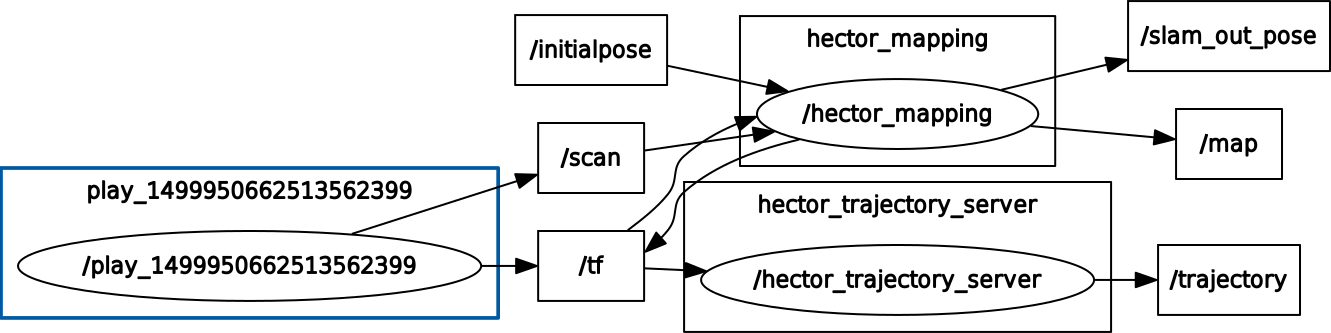
\includegraphics[width=1.\linewidth]{figures/hector_active_nodes}  
  \captionof{figure}{N\oe{}uds et topics d'intérêt et actifs lors de l'exécution d'Hector SLAM}
  \label{fig:hector}
\end{figure}

La figure \ref{fig:hector} expose les n\oe{}uds et topics actifs lors d'un l'utilisation d'\gls{Hector SLAM} à partir d'un jeu de données pré-enregistrées dans un fichier \gls{bagfile}.
Les n\oe{}uds actifs sont présentés au sein d'ellipses, les topics au sein de rectangles sous la forme \path{/<topic-name>} et les noms des packages auxquels les n\oe{}uds appartiennent figurent au dessus de chacun d'entre-eux. 
Enfin, les flèches signalent quels sont les n\oe{}uds responsables de la publication des topics, et quels sont les n\oe{}uds qui s'y sont inscrits. 
Le package généré par la lecture du \gls{bagfile} est représenté en bleu. 

On s'intéresse particulièrement aux topics en sortie d'\gls{Hector SLAM}. 
\path{/slam_out_pose} donne la localisation du robot en terme de position et d'orientation, \path{/trajectory} définit la trajectoire parcourue par le robot et \path{/map} donne la représentation de son environnement. 
Ce dernier topic correspond à une grille d'occupation, à savoir une discrétisation de l'espace sous forme de grille où chaque case porte la probabilité qu'elle soit un obstacle.
Dans la pratique la carte est de dimensions $2048 \times{2048}$ avec une résolution de $0.05m$. Les résultats issus de l'approche probabiliste s'expriment selon trois valeurs : $0$ pour une case vide, $1$ pour une case occupée et $-1$ pour une case inconnue. 
Chaque nouvelle acquisition attestant l'occupation d'une case augmente sa probabilté, et inversement lorsqu'une acquisition indique que la case est libre.
Lorsque la probabilité portée par une case dépasse un seuil interne à \gls{Hector SLAM}, la case sera considérée comme occupée et passera à la valeur $1$\footnote{Ce seuil est fixé à $0.5$}

L'intégration d'\gls{Hector SLAM} au projet s'est déroulée en plusieurs temps.
Nous avons d'abord pu prendre l'outil en main avant l'achat du \gls{LIDAR} grâce à l'utilisation de données de test contenues par des \gls{bagfile}. 
Durant cette étape, les résultats pouvaient être visualisés grâce à RViz, un outil graphique inclu dans \gls{ROS}\footnote{Pour la distribution Kinetic de ROS, RViz est présent dans les paquets d'installation dits ``Desktop''\cite{Bib_ROS_install}.}.
La figure \ref{fig:rviz} illustre le résultat obtenu pour un jeu de test issu de la RobotCup German Open 2011. 
Les zones non explorées y figurent en gris foncé, les zones explorées mais vides en gris clair et les zones occupées en noir. 
Le robot est resprésenté par trois composantes orthogonales de couleur bleue, verte et rouge et la trajectoire parcourue est une courbe rouge. 

Dans un deuxième temps, il a fallu adapter \gls{Hector SLAM} pour recevoir en entrée les données du \gls{LIDAR}, ce qui revient principalement créer des fichiers de lancement (\emph{launchfile})
adaptés au périphériques d'acquisition. Dans notre cas nous avons créé deux fichiers distincts : l'un pour le mode d'exécution standard et l'autre pour un mode ``debug''.
Nous avons également mis en place des éléments qui définissent les tranformations spatiales entre les différents périphériques et qui seront présentés dans la partie \ref{subsection:ROSnodes}. 

\begin{figure}[h]
  \centering
    \includegraphics[width=.4\linewidth]{figures/rviz}  
  \captionof{figure}{Visualisation avec RViz d'un jeu de données pré-enregistrées}
  \label{fig:rviz}
\end{figure}

\section{Réalisations et architecture logicielles}

  \subsection{Le réseau ROS complet}
  \label{subsection:ROSnodes}
  
\gls{Hector SLAM} a été intégré à un réseau \gls{ROS} plus large prennant en compte les spécificités de notre application. 
Il était entendu que l'\gls{IHM} ne serait pas inclue dans ce réseau et serait développée avec Qt Creator (voir partie \ref{subsection:Qt}).  

La définition du réseau doit alors s'inscrire comme une solution aux problématiques suivantes : 

\begin{itemize}
  \item le contrôle du \gls{LIDAR} ainsi que la lecture et l'émission des nuages de points calculés
  \item l'intégration d'\gls{Hector SLAM} 
  \item la communication des résultats de cartographie et de localisation vers l'\gls{IHM}
\end{itemize}

\begin{figure}[h]
  \makebox[\textwidth][c]{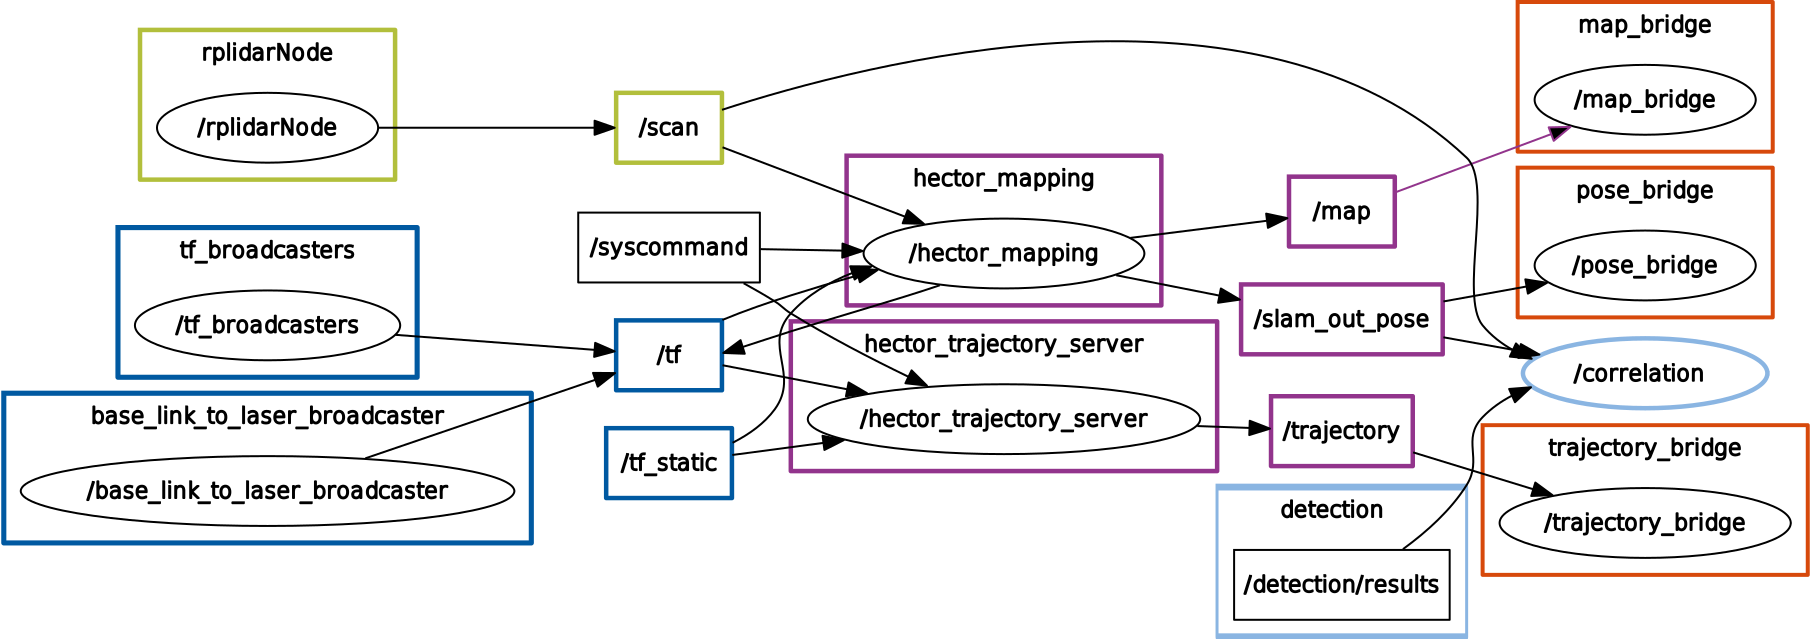
\includegraphics[width=1.1\textwidth]{figures/all_nodes}}%
  \captionof{figure}{Réseau ROS intégré au système}
  \label{fig:rosnet}
\end{figure}

Le premier point, représenté en vert sur la figure \ref{fig:rosnet}, est assuré par un n\oe{}ud embarqué sur le Raspberry Pi régissant la communication avec le \gls{LIDAR}.   
Il s'interface avec plusieurs fichiers d'en-tête qui constituent la \gls{SDK} du \gls{LIDAR}.
Cet élément du réseau \gls{ROS} est fourni par SLAMTEC dans son kit de développement.
Sa mise en \oe{}uvre a demandé de comprendre les principales méthodes de la \gls{SDK} et la portée fonctionnelle de chaque fichier d'en-tête. 
Par ailleurs, outre l'installation de \gls{ROS} sur Raspberry, la mise en place du matériel a nécessité l'installation d'un driver permettant la conversion des données 
depuis l'UART vers l'USB, ainsi que la définition de règles d'utilisation du port série sur lequel est raccordé le \gls{LIDAR}.
En sortie, ce n\oe{}ud publie le topic \path{/scan}, correspondant au format de messages \path{sensor_msgs/LaserScan} précédemment évoqué (voir \nameref{annexe:laserscan}). 

\begin{figure}[h]
  \centering
    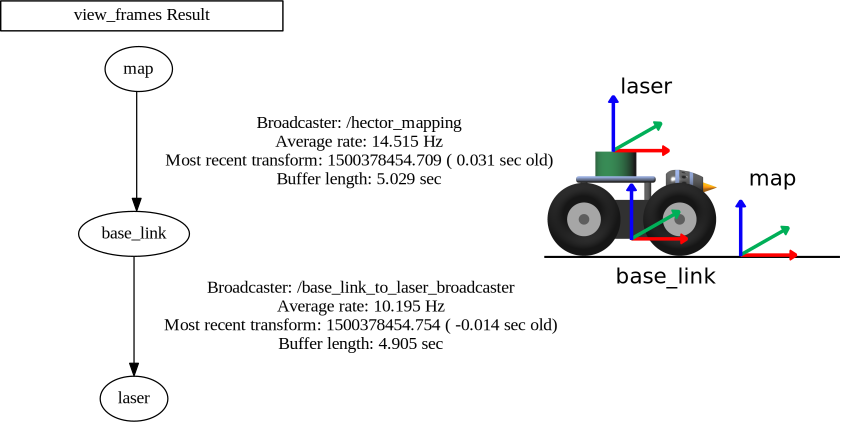
\includegraphics[width=1.\linewidth]{figures/frames_and_schema}  
  \captionof{figure}{Systèmes de coordonnées et transformations au sein du système}
  \label{fig:frames}
\end{figure}

L'intégration d'Hector SLAM demande la définition de plusieurs systèmes de coordonnées correspondant au divers périphériques d'intérêt.
Les transformations spatiales entre ces systèmes étant également requises par \gls{Hector SLAM}, elles sont publiées au travers d'un package appelé \gls{tf}\cite{Bib_ROS_tf}\cite{Bib_tf}. 
Les n\oe{}uds et topics impliqués dans ce processus sont représentés en bleu foncé sur la figure \ref{fig:rosnet}. 
\gls{tf} distingue deux types de transformations : les transformations statiques et les transformations dynamiques. 
Dans le premier cas, il suffit de définir l'identifiant d'un repère de référence (\emph{frame\_id}) et d'un repère fils (\emph{child\_frame\_id}) ainsi que la transformation que subit ce dernier, en s'assurant qu'elle ne sera jamais amenée à changer.
Dans le second cas, il faut généralement passer par la création d'un noeud publiant la valeur de ce décallage régulièrement durant l'exécution. 
Pour mieux saisir les enjeux soulevés par l'intégration d'\gls{Hector SLAM}, la figure \ref{fig:frames} donne les systèmes de coordonnées définis, 
ainsi que les n\oe{}uds implémentés (les \emph{broadcasters}) responsables de la publication des transformations. 

Le système \emph{map} est un repère fixe, ancré au sol, qui sert de référence au positionnement du robot sur le long terme\cite{Bib_frames}.
\emph{base\_link} est un repère mobile par rapport à \emph{map} attaché sous la plateforme mobile en son centre. Une première transformation entre \emph{map} et \emph{base\_link} est requise par \gls{Hector SLAM}. 
Elle est calculée par le n\oe{}ud \path{/tf_broadcasters} (voir figure \ref{fig:rosnet}) à partir des relevés odométriques fournis par le robot.
Une fois intégrée par \gls{Hector SLAM}, cette transformation est corrigée puis ré-émise par \path{/hector_mapping} : c'est le topic \path{/tf} de la figure \ref{fig:rosnet}. 
Enfin, le n\oe{}ud \path{/base_link_to_laser_broadcaster} publie régulièrement la transformation entre \emph{base\_link} et \emph{laser}, c'est-à-dire le différentiel de position entre la base du robot et le \gls{LIDAR}. 
Celui-ci n'étant jamais amené à changer nous sommes dans le cas d'une transformation statique définie de la manère suivante dans le launchfile d'Hector SLAM en mode d'exécution 
standard\footnote{En mode ``debug'' cette transformation est non avenue puisqu'elle est déja comprise le \emph{bagfile} responsable du rejeu des données} : 

\begin{lstlisting}[style = custombash]
<!-- Laser is set 25cm above robot base. Node arguments must be : 
dx dy dz yaw pitch roll frame_id child_frame_id publishing_frequency_in_ms 
-->

<node pkg="tf" type="static_transform_publisher" 
      name="base_link_to_laser_broadcaster" 
      args="0 0 0.25 0 0 0 base_link laser 100" />  
\end{lstlisting}

Nous obtenons ainsi un moteur de SLAM fonctionnel à partir duquel nous devons construire une \gls{IHM}. 
Pour ce faire, nous avons défini trois n\oe{}uds appelés \emph{bridges} représentés en orange sur la figure \ref{fig:rosnet}. 
Chacun d'entre-eux s'abonne à l'un des topics en sortie d'\gls{Hector SLAM}, 
Ensuite, les données utiles sont formatées par appel à une classe statique nommée \path{Serializer} et communiquées à l'\gls{IHM} par le biais d'un client \gls{TCP} implémenté avec l'API socket. 
La sérialisation répond à un schéma générique composé d'une en-tête (\emph{header}) et d'une charge utile (\emph{payload}). Il est représenté sur la figure \ref{fig:buffer}. 

\begin{figure}[h]
  \centering
    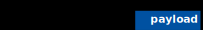
\includegraphics[width=.5\linewidth]{figures/buffer}  
  \captionof{figure}{Définition du paquet générique de transmission de données à l'IHM}
  \label{fig:buffer}
\end{figure}

Les éléments contenus par le header sont \path{tID}, un identifiant donnant le type de la donnée transmise, \path{pSize}, la taille du payload et un \path{padding} à $0$ qui vise à ce que le \emph{header} atteigne 20 octets. 
La formation du \path{payload} dépend quant à elle des données à tansmettre. 
La principale difficulté réside en la transmission de la grille d'occupation contenue par le topic \path{/map}. 
Celle-ci contenant plus de $4$ $000$ $000$ valeurs entières, nous nous sommes focalisés sur l'émission de mises à jour locales à chaque acquisition, plutôt que globales\footnote{Il en va de même pour la trajectoire où,
dans un même souci d'optimisation, nous effectuons un différentiel entre les valeurs précédemment acquises et la nouvelle acquisition}. 
Ainsi, le \path{payload} se construit de la manière suivante afin de désencombrer la bande passante et réduire la taille de la structure de données qui l'encapsule. 

\newpage

\begin{lstlisting}[style = customcpp]
// Fill a buffer with occupancy grid local updates
int Serializer::serializeMap( const nav_msgs::OccupancyGrid& map, 
							  const nav_msgs::OccupancyGrid& old_map, 
							  std::string *buffer ) {
	
	std::string header, payload; 
	
	// Check data consistency  
	if(map.info.width != old_map.info.width || 
	   map.info.height != old_map.info.height) {
		std::cout << "Serialization error : Map and old_map with different dimensions" << std::endl; 
		return -1; 
	}	
	
	// Fill payload with updated cases' value and index
	for(int i = 0; i < map.info.width * map.info.height; ++i) {
		if(map.data[i] != old_map.data[i])	
		    payload.append( std::to_string(i) + ","
				    + std::to_string(map.data[i]) + "," );	
	}	
	payload.append( "EOP" );
	
	// Fill header, return error if its size exceeds 20 bytes
	header.append( MAP_ID );
	header.append( "," + std::to_string(payload.length()) + "," );
	if( Serializer::addZeroPadding(&header) < 0 ) return -1; 
	
	// Fill buffer with header and payload 
	buffer->append( header );
	buffer->append( payload );	
	return 0; 
}
\end{lstlisting}

Enfin, la figure \ref{fig:rosnet} fait également état du n\oe{}ud \path{/correlation} abonné aux résultats de détection d'objets d'intérêt et au topic \path{/scan}.
Il est responsable du croisement de ces données afin de déterminer, quand cela est possible, les coordonnées d'un objet détecté à partir du flux vidéo.  
La technique employée ici consiste à trouver pour chaque résultat de détection, la position du robot à l'instant de la détection ainsi que les faisceaux du LIDAR susceptibles d'avoir atteint l'objet. 
Lorsque ces 
derniers existent\footnote{Le plan parcouru par les faisceaux du LIDAR doit être compris entre les extrémités haute et basse de l'objet.} nous devons transformer la distance et l'angle associés dans le système de coordonnées de la carte. 
L'algorithme suivant donne les principes implémentés à cet effet. 
\\
\IncMargin{1em}
\begin{algorithm}[H]
 \caption{Algorithme de calcul des résultats de corrélation}
 \BlankLine
 \Entree{	$R$ les derniers résultats de détection reçus sous la forme : dimensions plane de l'objet $(w, h)$ et ses coordonnées sphériques $(\phi, \theta)$ \\
	$t$ un entier non signé, estampille de $R$ }
	
 \BlankLine	
 \Donnees{ $S$ l'ensemble des scans n'ayant jamais été corrélés \\ 
	  $P$ l'ensemble de positions du robot n'ayant jamais été corrélées\\
	  $scan$ un timestamp et un ensemble $coord$ de paires de coordonnées polaires $(\theta, r)$\\
	  $pose$ un timestamp, une position $p = (x, y, z)$ et une orientation $ q = (pitch, roll, yaw)$ \\
	  $angle$ l'angle auquel se trouve l'objet dans le système de coord. du scan \\
	  $matched$ couple $(\theta, r)$ caractérisant la position de l'objet détecté}
 \BlankLine
 \Deb
 {
  \eSi{$S = \emptyset \vee P = \emptyset$}
  {
    \Retour{-1}
  }
  {
    \tcc{find temporally nearest scan and pose with respect to $t$}
    $scan \leftarrow findNearestScan(t)$ \\
    $pose \leftarrow findNearestPose(t)$ \\
    \eSi{$scan = 0 \vee pose = 0$}
    {
      \Retour{-1}
    }
    {
      \Pour{$r \in R$}
      {
      \tcc{check if current object $r$ crosses LIDAR laser}
	\Si{$(r.theta - \dfrac{r.h}{2} < \dfrac{\pi}{2}) \land (r.theta + \dfrac{r.h}{2} > \dfrac{\pi}{2})$}
	{
	  $angle \leftarrow r.phi$ \\
	  \Pour{$s \in scan.coord$}
	  {
	    \Si{$s.\theta > angle$}
	    {
	      \textbf{break}
	    }
	    $matched \leftarrow s$
	  }
	  \tcc{add object position and dimension in result structure}
	  \Si{$matched.r \neq \infty$}
	  {
	    $r.x \leftarrow pose.p.x + matched.r \times \cos(\ matched.\theta + pose.yaw\ )$\\
	    $r.y \leftarrow pose.p.y + matched.r \times \sin(\ matched.\theta + pose.yaw\ )$\\
	    $r.z \leftarrow LIDAR\_LENGTH + matched.r \times \tan(\ \dfrac{\pi}{2} - r.\theta\ )$\\
	    $r.w \leftarrow 0.5 \times 2 \times matched.r \times \tan(\ \dfrac{r.w}{2}\ )$ \\
	    $r.h \leftarrow 0.5 \times 2 \times matched.r \times \tan(\ \dfrac{r.h}{2}\ )$ 
	  }
	}
      }
      \Retour{1}
    }
  }
}
\end{algorithm}

  \subsection{Interface Homme-Machine avec Qt Creator}
  \label{subsection:Qt}
  
L'Interface Homme-Machine de l'application a été implémentée en C++ avec l'\gls{API} Qt, facilitant notamment la réalisation de l'interface graphique au moyen de l'environnement de développement Qt Creator. 
Dans l'\gls{API} Qt, les éléments graphiques sont appelés \emph{widgets} et dérivent de classes définies dans les bibliothèques internes, telles que \path{QWidget}, \path{QOpenGLWidget} ou encore \path{QDialog} pour ne citer 
que celles qui ont été utiles au projet.  
Qt fourni également un mécanisme de communication inter-classes thread-safe et type-safe, par le biais d'éléments appelés signaux et 
slots\footnote{Ce mécanisme peut être mis en parallèle avec les callbacks en C ou C++ ou encore les signaux fournis par l'API boost en C++}.
Ceux-ci ont la particularité d'occulter la démarche de liaison entre les parties communicantes et ne nécessitent pas de classe dédiée à cet effet. 
Ils permettent de mettre en place simplement des connexions \emph{one-to-many}, \emph{many-to-one} ou encore \emph{many-to-many}.
Un signal est une signature de fonction membre d'une classe, qui pourra être émis par ses instances. Les slots sont quant à eux des fonctions membres désignées par la macro Q\_SLOTS. 
La mise en \oe{}uvre de signaux et de slots est illustrée dans l'exemple suivant, tiré du code source du projet. 

\begin{lstlisting}[style=customcpp]
// sensorDataAvailable signal connection to setWifibotInfo slot
QObject::connect( wc_, &WifibotClient::sensorDataAvailable, 
				  w_, &MainWindow::setWifibotInfo );
\end{lstlisting}

\begin{lstlisting}[style=customcpp]
// signal emission in WifibotClient class
emit sensorDataAvailable(robotSensors);
\end{lstlisting}

\begin{lstlisting}[style=customcpp]
// data computing in MainWindow callback
void MainWindow::setWifibotInfo(SensorData sd)
{
    // dispatch info to sensor widgets through other signals and slots mecanisms
    emit setIRLeftValue(sd.IRLeft);
    emit setIRRightValue(sd.IRRight);
    emit setBatteryValue(sd.batVoltage);
    emit setOdomLeftValue(sd.odometryLeft);
    emit setOdomRightValue(sd.odometryRight);
    emit setSpeedLeftValue(sd.speedFrontLeft);
    emit setSpeedRightValue(sd.speedFrontRight);
}
\end{lstlisting}

\begin{figure}[h]
  \centering
    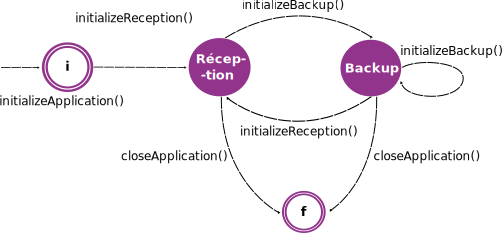
\includegraphics[width=.7\linewidth]{figures/state_machine}  
  \captionof{figure}{Machine à état de l'application Qt}
  \label{fig:stateMachine}
\end{figure}

D'un point de vue formel, le fonctionnement de l'application est régi par une machine à états relativement simple, représentée figure \ref{fig:stateMachine}.
Ces états facilitent la gestion des instances utiles à n'importe quel instant de l'exécution en dissociant clairement ce qui est du ressort de chacun des modes de fonctionnement définis. 
Le mode \emph{Réception} satisfait l'exigence principale du projet, à savoir présenter en temps-réel les résultats de \gls{SLAM} tout en assurant le contrôle du robot. 
Le mode \emph{Backup} répond à une fonctionnalité additionnelle offrant la possibilité à l'utilisateur de rejouer des données précédemment enregistrées. 
Le passage d'un état à l'autre est symbolisé par des flèches portant le nom de la méthode invoquée à cet effet.
Ces méthodes visent à libérer la mémoire relative aux ressources dynamiques du mode courant, à instancier correctement les ressources graphiques ou de contrôle propres au mode requis et finalement, à changer une variable représentant 
l'état du système. 
On note que les fonctions de transition sont des slots atteints par des interactions spécifiques de l'utilisateur sur la fenêtre graphique. 

\begin{figure}[h]
  \makebox[\textwidth][c]{\includegraphics[width=1.1\textwidth]{figures/ihm-model}}%
  \captionof{figure}{Modèlisation logicielle de l'Interface Homme-Machine}
  \label{fig:modelIHM}
\end{figure}

La figure \ref{fig:modelIHM} expose quant à elle les classes et packages développés avec Qt pour répondre aux exigences fonctionnelles et d'interface précédemment formulées.   
Sont également représentés les moyens de communications mis en place entre l'IHM et les autres éléments constituant le projet : le réseau \gls{ROS} et la couche d'exploitation du Wifibot.

Le point d'entrée de l'application est la classe \path{main.cpp} qui instancie la fenêtre principale de l'application \path{MainWindow}\cite{Bib_qmainwindow} et une classe \path{Apploader} spécifique à notre architecture.
Cette dernière maintient et met à jour la machine à états présentée en \ref{fig:stateMachine} gérant ainsi le cycle de vie de toutes les autres instances.  

Le package \emph{SLAM} traite les données en sortie du réseau \gls{ROS}. \\
La classe \path{ROSBridgesServer} instancie un serveur \gls{TCP} consacré à la communication avec les n\oe{}uds de \emph{bridge} décrits dans la partie \ref{subsection:ROSnodes}. 
Ces données sont ensuite transmises à des contrôleurs dédiés à chaque type de données (carte, position ou trajectoire) qui assurent le parsing des paquets reçus puis émettent des signaux aux \emph{widgets} de rendu. 
Dans notre cas, deux \emph{widgets} sont susceptibles de rendre ces données : \path{SlamWidget} ou \path{SlamBackupWidget} respectivement associés au mode \emph{Réception} ou \emph{Backup}.
Ces \emph{widgets} héritent de la classe Qt \emph{QOpenGLWidget} fournissant les fonctionnalités de rendu graphique d'OpenGL dans un contexte Qt. 
La figure \ref{fig:reception} donne un apperçu de l'\gls{IHM} en mode \emph{Réception} afin de présenter les différents éléments de l'application. 
La fidélité des résultats sera quant à elle discutée dans la partie \ref{chap:bilan}.  

\begin{figure}[h]
  \centering
    \includegraphics[width=1.\linewidth]{figures/slam-widget}  
  \captionof{figure}{Rendu visuel de l'IHM en mode Réception}
  \label{fig:reception}
\end{figure}

Nous pouvons visualiser la fenêtre principale (\path{MainWindow}) complétée d'instances de \emph{widgets} responsables du rendu d'éléments d'intérêt : 
\begin{itemize}
 \item \textbf{un widget de rendu OpenGL}, en bleu, fourni une représentation de la carte, du robot par le biais d'un modèle 3D et de sa trajectoire (position et orientation en tout temps)
 \item \textbf{un panneau de contrôle}, en vert, est découpé en quatre sections : le Wifibot, le réseau ROS, un joystic virtuel et une console de logs 
 \item \textbf{une barre de menu}, en jaune, permet la sauvegarde de jeux d'acquisition, le chargement d'une sauvegarde pour la rejouer, l'édition de paramètres de l'application ou l'affichage du manuel utilisateur
\end{itemize}

La figure \ref{fig:replay} expose le rendu global en mode \emph{Backup}. 
Celui-ci se distingue particulièrement du mode d'acquisition par la présence --au sein du panneau de contrôle-- d'un \emph{player} offrant les fonctionnalités d'un lecteur multimédia classique.

\begin{figure}[h]  
  \centering
    \includegraphics[width=1.\linewidth]{figures/slam-backup}  
  \captionof{figure}{Rendu visuel de l'IHM en mode rejeu}
  \label{fig:replay}
\end{figure}

\`{A} cet effet, un format d'enregistrement des données propre à l'application a été défini en \gls{XML}.
Ce format, appelé \emph{DOG}\footnote{Pour Detection and Occupancy Grid} est géré par les classes du package \path{DogFiles} : \path{DogFilesWriter} pour l'écriture et \path{DogFilesParser} pour la lecture. 
Des techniques de compressions ont été appliquées pour les données de taille critique devant être sauvegardées. 
Ainsi, les données décrivant la carte sont traitées par un algorithme d'encodage par répétition (Run Lenght Encoding) tandis que toutes les composantes des vecteurs de trajectoire du robot sont gérées par la méthode suivante :

\begin{lstlisting}[style=customcpp]
// Multiply entry by 100, truncate it and returns its hexadecimal value. Negative number are concatenated with '-' char and encoded like positive values.
QString SlamWidget::floatToHex(float v)
{
    return (int)(v * 100) >= 0.0f
            ? QString::number( (int)(v * 100), 16 )
            : QString('-' + QString::number( (int)-(v * 100), 16 ));
}
\end{lstlisting}

Un algorithme similaire a été appliqué pour l'ensemble des orientations du robot. 
Ces techniques ont permis de réduire significativement les données à sauvegarder à l'aide d'une compression sans perte dans un  premier cas et une perte de l'ordre du centième de case (soit 0.0005 m) dans un second cas.  
  
  \subsection{\'{E}léments de modularité mis en place}
  
La réalisation de l'application a d'emblée été associée à un objectif de modularité afin d'appréhender au mieux la perspective de stages futurs et / ou d'une possible adaptation industrielle du projet. 
L'utilisation de ROS allant dans ce sens, il paraissait intéressant d'appliquer ce principe à l'\gls{IHM}, tant dans l'architecture du logiciel qu'au travers des fonctionnalités proposées à l'utilisateur final. 

Le premier point se retrouve principalement dans l'implémentation de l'\path{Apploader} qui gère le cycle de vie des instances d'une manière communément compréhensible : création, mise-à-jour puis destruction.  
D'autre part, l'interface graphique et les éléments de communication avec les n\oe{}uds peuvent eux-mêmes être modifiés à convenance par le biais de l'\gls{IHM}. 
Nous exposons ici les principes qui sous-tendent cette démarche, nous amenant à balayer les points suivants : 

\begin{itemize}
  \item le paramétrage modulaire du réseau ROS
  \item les éléments graphiques attestant l'état de chaque n\oe{}ud
  \item le contrôle du réseau ROS depuis l'IHM
\end{itemize}

Qt offre un système de paramétrage des applications qui s'appuie sur des fichiers au format texte et sur une classe \path{QSettings} indépendante de la plateforme utilisée
\footnote{En l'occurence, sur un système Unix, de tels fichiers seront stockés au format \path{.ini} sous \path{~/.config/<filename>.ini}}.
Cette dernière permet l'écriture de paramètres selon le paradigme clé / valeur et hiérarchisés sous forme de groupe.  
Dans notre IHM, une classe statique \path{SettingsManager} est utilisée pour écrire de tels paramètres, soit à l'initialisation de l'application soit lors de la configuration de celle-ci par l'utilisateur. 
Nous avons défini les groupes suivants relativement au réseau ROS :

\renewcommand*\DTstylecomment{\rmfamily\color{red}}
\dirtree{%
.1 ros\DTcomment{groupe de paramétrage du réseau ROS}. 
.2 $<$ID$>$\DTcomment{identifiant du groupe de paramètres}. 
.3 package. 
.4 $<$nom du package$>$\DTcomment{nom du package à invoquer}. 
.3 lauchfile. 
.4 $<$launchfile$>.$launch\DTcomment{nom du launchfile à invoquer}. 
.3 islocalnode. 
.4 $<$bool$>$\DTcomment{indique si le noeud est local ou embarqué}. 
.3 label. 
.4 $<$GUI label$>$\DTcomment{label à afficher sur l'interface}. 
.3 nodes. 
.4 node. 
.5 $<$liste de noeuds$>$\DTcomment{liste de noeuds à stopper}. }

L'utilisateur peut mettre à jour ou supprimer les valeurs par défaut et créer de nouvelles entrées directement depuis l'application sous \path{Edit > Settings > ROS} (voir figure \ref{fig:settings}).

\begin{figure}[h]
  \centering
    \includegraphics[width=.7\linewidth]{figures/settings}  
  \captionof{figure}{Boîte de dialogue de configuration du réseau ROS depuis l'IHM}
  \label{fig:settings}
\end{figure}

Ces paramètres sont ensuite parsés, permettant la présentation et l'utilisation de chaque module ROS de manière uniforme.
D'un point de vue graphique, la classe \path{GuiControl} est responsable de la création dynamique des éléments de l'interface représentant les modules ROS, à partir de la clé de configuration \path{ros/<ID>/label/<GUI label>} 
tels que représentés figure \ref{fig:guicontrols}.

\begin{figure}
  \centering
    \includegraphics[width=.3\linewidth]{figures/guicontrols}  
  \captionof{figure}{Contrôle du réseau ROS créé dynamiquement sur l'interface graphique}
  \label{fig:guicontrols}
\end{figure}

Parallèlement, chaque nouvel identifiant sous \path{ros/<ID>} entraine l'instanciation de la classe \path{NodesLauncher} ou \path{NodesLauncherOverSSH} --en fonction du caractère local ou non du package-- et de la classe 
\path{NodesKiller}. 
Ces objets exécutent un shell Linux (\path{/bin/bash}) au sein d'un membre Qt de type \path{QProcess} permettant l'éxecution du launchfile afférent lorsque l'utilisateur presse le bouton ``Start'' du module.
Ils sont aussi responsables de la redirection des sorties du processus vers les sorties dédiées à la journalisation des évènements de l'application\footnote{La classe \path{LogsHandler} est utilisée pour journaliser les messages d'une part dans des fichiers datés du répertoire d'exécution 
de l'application et d'autre part, dans la console du panneau de contrôle}. 
La classe \path{NodesKiller} va quant à elle émettre des commandes système vers le ROS Master afin de tuer les n\oe{}uds d'un package lorsque l'utilisateur souhaitera mettre fin à leur exécution. 

Pour résumer, un utilisateur voulant ajouter un nouveau package ROS à l'application devra le compiler de manière classique dans son workspace Catkin, éditer un \emph{launchfile} permettant d'éxecuter le ou les n\oe{}uds afférents puis
simplement renseigner les informations requises depuis l'IHM. 
Sous la section \path{Edit > Settings > Network} l'utilisateur pourra également configurer les noms d'hôtes et adresses IP distants, adaptant ainsi le système à d'autres modèles ou instances de robots. 
Si l'opérateur venait à utiliser une plateforme dotée de capteurs communiquant leurs résultats à un package ROS dédié, le contrôle de ces nouveaux éxecutables pourrait être couvert par l'application en quelques manipulations seulement.  
  \chapter{Bilan et perspectives}
\label{chap:bilan}

\section{Organisation du travail}
\label{sec:orga}
  \subsection{Application du référentiel qualité interne}
  \label{sec:qualite-interne}

  Nous exposons ici les éléments fournis par SII ayant guidé de manière significative la conduite du projet. 
  Ceux-ci seront plus ou moins détaillés en fonction du temps consacré à leur mise en place.
  
    \begin{figure}[h]
    \centering
      \includegraphics[width=.6\linewidth]{figures/rel-fonctions}  
    \captionof{figure}{Modèle de définition des modules logiciels et relations entre leurs fonctions}
    \label{fig:rel-fonctions}
  \end{figure}
  
  Les premiers éléments oraganisationnels qui ont été formalisés s'incarnent par deux documents de spécification appelés \gls{STBL} et \gls{DCL}.
  Le premier vise, comme son nom l'indique, à exprimer le plus objectivement possible le besoin qui justifie la réalisation logicielle, notamment au moyen d'exigences représentées figure \ref{fig:exigences}. 
  Cette énumération haut-niveau permet d'appréhender simplement et rapidement le périmètre du logiciel ciblé. 
  Cependant, la réalisation de ce document en bonne et dûe forme nécessite une liste exaustive d'exigences fonctionnelles vues comme des ensembles de fonctions qu'il convient de décrire en terme de rôle, d'entrées, de sorties et
  de traitements. 
  Dans le cadre de ce stage, nous définissons des fonctions comprises dans des modules distincts et étant reliés comme présenté sur la figure \ref{fig:rel-fonctions}.
  Puis, pour chacune des fonctions, on va définir des sous-fonctions, idéalement jusqu'à un niveau de granularité maximal où tous les types de données sont énumérés. 
  Par exemple, on établit que la fonction \emph{Transmettre} du module \textbf{\textcolor{red-stbl}{Map\_bridge}} regroupe les trois sous-fonctions \emph{Recevoir un message}, \emph{Formater un message} et \emph{\'{E}mettre un message}. 
  Afin d'illustrer cette démarche, nous donnons ici pour exemple la spécification de la fonction \emph{Transmettre : Formater un message}. 
  
  \textbf{1. Rôles } \\
  Cette fonction est activée à l’arrivée d’une demande de traitement de message sur la liaison SLAM $\Longleftrightarrow{}$ MAP\_BRIDGE.
  Elle intervient après que la fonction de réception ait attesté de la consistance du message reçu.
  Elle permet d’extraire la charge utile du message reçu et d’en réduire significativement le volume avant envoi.  Les données en sorties sont sérialisées.
  Cette extraction s’effectue en comparant OCCUPANCY\_GRID avec une copie locale de la dernière carte reçue OLD\_OCCUPANCY\_GRID.
  
  \textbf{2. Entrées }
  \begin{figure}[!h]
    \begin{center}
      \begin{tabular}{|l|l|}
	\hline
	\textbf{Désignation} & \textbf{Type de données} \\
	\hline
	Message OCCUPANCY\_GRID & OccupancyGrid \\
	\hline
      \end{tabular}
    \end{center}
    \caption{Entrées de la fonction \emph{Transmettre : Formater un message}}
  \end{figure}
  
  \textbf{3. Sorties }
  \begin{figure}[!h]
    \begin{center}
      \begin{tabular}{|l|l|}
	\hline
	\textbf{Désignation} & \textbf{Type de données} \\
	\hline
	Message MAP & OccupancyGridUpdate \\
	Message INI\_MAP & IniOccupancyGrid \\
	\hline
      \end{tabular}
    \end{center}
    \caption{Sorties de la fonction \emph{Transmettre : Formater un message}}
  \end{figure}
  
  Notons que la spécification des types de données d'entrées-sorties est donné dans un document externe. 
  Relativement à l'exemple précédent, le type d'OCCUPANCY\_GRID est décrit en \nameref{annexe:occupancygrid}.  
  
  \textbf{4. Traitements }
  
  \textbf{NB} : Les traitements sont idéntifiés de manière unique au sein d'un document, ils satisfont également des règles permettant d'être traités automatiquement par des logiciels de suivi de projet. 
  Nous donnons ici un exemple succint permettant d'en saisir le sens. Dans la pratique une sous-fonction donne lieu à plusieurs traitements.
  
  \textbf{$[$REQ\_STBL\_MAP\_BRIDGE\_FORM\_1$]$}
  
    \hspace{10mm} Si OLD\_OCCUPANCY\_GRID existe : 
    
    \hspace{10mm} On compare le champ ``data'' de OCCUPANCY\_GRID et de 
    \\ OLD\_OCCUPANCY\_GRID. 
    
    \hspace{10mm} On crée la structure MAP à partir des valeurs de ``data`` qui diffèrent. 
    
    \hspace{10mm} MAP est une chaîne de caractères dont les valeurs sont séparées par des ",".\\ 
  \textbf{$[$FIN\_REQ$]$}
  
  Le Document de Conception Logicielle est quant à lui intervenu plus tard dans l'avancée du stage. 
  Il consiste à formaliser les éléments conceptuels, en termes d'architecture physique et logicielle du projet. 
  Ces briques ayant été largement explicitées au long de ce rapport nous n'attayerons pas d'avantage ce point. 
  
  Par ailleurs, un planning présentant une granularité hebdomadaire a été effectué au mois de mars, ce document est présenté en \nameref{annexe:planning}.
  Cette réalisation vise à définir et ordonnancer les tâches à réaliser et, d'autre part, à estimer l'impact temporel de chacune d'entre-elles. 
  Ce document a été réalisé dans une optique d'organisation personnelle mais a également constitué un outil d'évaluation et de communication avec M. Daumand qui a été en grande partie affecté en missions hors de l'agence. 
  Il s'agissait donc pour nous de fixer les jalons clés, les \emph{dead-lines} et les versions du logiciel à produire afin qu'il suive de manière pragmatique l'avancée du travail. 
  
  \subsection{Vers une conduite AGILE adaptée}
  
  Au référentiel interne de qualité du logiciel se sont ajoutées certaines bonnes pratiques issues de la formation en Architecture et Sécurité du Logiciel prodiguée à l'INSA Centre Val-de-Loire.
  En particulier, nous avons utilisé le gestionnaire de versions Git au travers du système de gestion de dépôts (forge) GitLab auquel nous avons appliqué une stratégie de création de branches dite \og Git Flow \fg{}.
    \begin{figure}[h]
    \centering
      \includegraphics[width=.6\linewidth]{figures/gitflow}  
    \captionof{figure}{Politique de gestion de branches Git adoptée}
    \label{fig:gitflow}
  \end{figure}
  Ce modèle d'utilisation de Git vise à minimiser les conflits et les régressions, accentuer la visibilité des tâches en cours ou terminées et à scinder clairement les phases de développement du logiciel. 
  \`{A} cet effet nous avons adopté la démarche illustrée sur la figure \ref{fig:gitflow} qui se lit de bas en haut et où les commits sont représentés par des points.
  Cela consiste à travailler sur une branche de développement (\path{develop}), à partir de laquelle nous créons une branche par fonctionnalité (\path{feature}), éventuellement une branche \path{hotfix} pour une correction de bug
  et, enfin, une branche \path{realease} qui va aboutir sur la dernière version stable du logiciel.
  Cette branche est ensuite répercutée sur \path{develop} et \path{master}, dans le premier cas  pour continuer les actions de développement et dans le second, afin de permettre la récupération des sources ou leur déploiement. 
  
  Aussi, l'\path{Apploader} a constitué une refonte majeure de l'architecture du logiciel qui a été conceptualisée et développée en équipe. 
  Afin de répartir les tâches que nécessitait son implémentation, nous avons pu expérimenter l'utilisation d'un \gls{Kanban} recensant : 
  
  \begin{itemize}
   \item les tâches à effectuer, par exemple \emph{Enregister les données de cartographie dans le format DOG}
   \item la compléxité relative de chacune d'entre-elles 
   \item les dépendances de certaines tâches les unes par rapport aux autres
  \end{itemize}

  Définir la \og complexité \fg{} d'une tâche revient à lui attribuer un score en se référant aux scores attribués pour les tâches précédentes. 
  Les méthodes AGILES --notamment \gls{SCRUM}-- préconnisent le recours à des échelles de quantification relatives plutôt qu'à des jours hommes ou d'autres échelles se voulant précises. 
  Concrètement on peut utiliser les valeurs de la suite de Fibonacci qui suivent ce que l'on appelle la courbe d'incertitude, à savoir qu'au plus une valeur est élevée, au plus l'écart avec la valeur suivante sera grande. 
  Nous avons estimé la complexité des unités de travail à réaliser selon une méthode également empruntée à SCRUM, appelée \emph{planning poker}. 
  Tous les participants disposent d'un jeu de carte qui, dans notre cas, comporte les nombres $\dfrac{1}2, 1, 2, 3, 5, 8, 13, \infty$. 
  L'effort de réalisation est ensuite estimé en même temps pour une tâche donnée, puis soumis à discussion dans le cas de désaccord. 
  Cette pratique est à la fois rapide, ludique et présente l'intérêt de dénuer d'emblée la quantification de l'influence mutuelle des participants. 
  
  Ce Kanban a ainsi été adopté dans une optique d'ordonnancer les tâches et, accessoirement, de les répartir entre les membres de l'équipe. 
  Il a aussi permis d'attester visuellement de nos avancées respectives et du nombre de tâches en cours permettant un allègement ou une répartition de la charge si besoin.
  La consultation du nombre de tâches restantes a également joué dans nos décisions de poursuivre telle ou telle fonctionnalité au profit d'autres. 
  
\section{Résultats en vue d'un prolongement}  
  \subsection{Un module de SLAM en adéquation avec les attentes du projet}
  
  Nous nous intéressons dans un premier lieu à la fidélité des résultats de SLAM et dans un second temps, à une appréciation de l'ensemble du projet, incluant également les travaux d'Alban Chazot et bien sûr la vision de M. Daumand.  
  
  La figure \ref{fig:carto} donne un apperçu de la précision des résultats de SLAM. 
  Elle met en parallèle les résultats cartographiques du système avec un plan d'évacuation des locaux dans lesquels l'acquisition a pu être menée. 
  Pour des raisons pratiques, toutes les pièces n'ont pu être scannées, puisque celles-ci hébergent des collaborateurs ou directeur d'agence menant leurs activités.
  
  \begin{figure}[h]
    \centering
      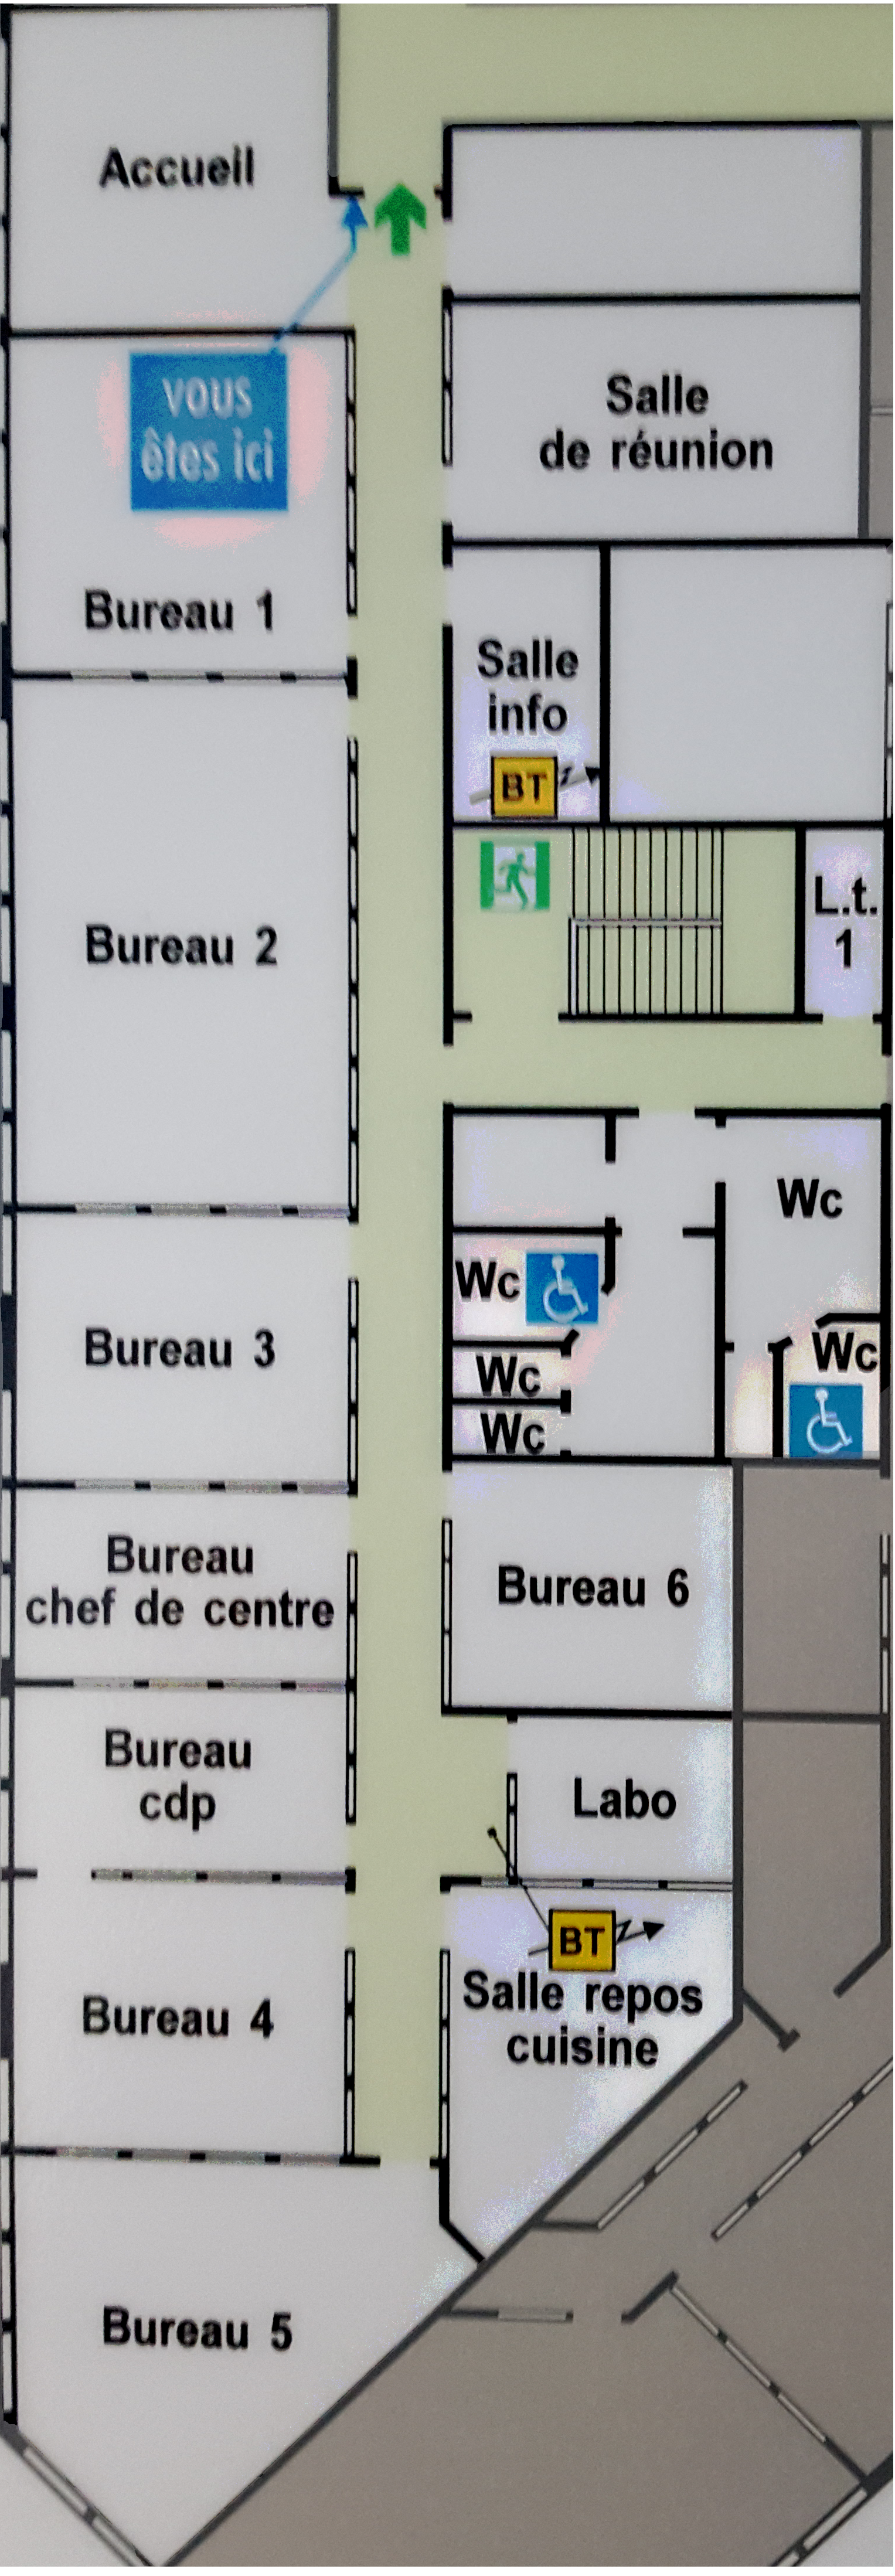
\includegraphics[width=1.\linewidth]{figures/plan}  
    \captionof{figure}{\`{A} gauche cartographie des locaux avec le logiciel, à droite plan d'évacuation correspondant}
    \label{fig:carto}
  \end{figure}
  
  Le plan des locaux est complété par des cercles de couleur verte pour les pièces qui ont été au moins à moitié explorées et de couleur orange pour les pièces visibles à moins de $50\%$. 
  Enfin nous représentons sur fond gris les pièces qui n'ont pas été scannées du tout. 
  Le couloir central a été parcouru dans toute sa longueur et la porte d'entrée est pointée par une flèche noire sur les deux représentations, afin d'éviter toute confusion quant à la façon de les interpréter. 
  
  On remarque empiriquement que les lieux cartographiés sont reconnaissables sans trop de difficultés, que leur agencement correspond à la réalité perçue et que les proportions des salles sont pour la plupart fidèles. 
  On peut aussi noter la précision du rendu des obstacles fixes : portes, pieds de tables, de chaises ou du baby-foot situé au centre de l'accueil dont trois pieds sur quatre sont visibles et correctement situés. 
  La géométrie des murs est également respectée, ce qui peut être attesté par les angles droits des pièces ou la régularité du couloir. 
  
  Cependant le résultat n'est pas sans défauts et certaines erreurs méritent d'être discutées. 
  L'imperfection la plus flagrante se situe au niveau du bureau 2. 
  Selon la cartographie celui-ci est aussi long que le bureau 3, tandis qu'il est, dans les faits, presque deux fois plus long. 
  Cette déformation se retrouve en effet sur toutes les acquisitions qui se sont déroulées de la manière suivante : 
  \begin{itemize}
   \item départ du bureau 3
   \item sortie du bureau 3 en direction du bureau 2
   \item déplacement dans un couloir de 8 mètres
   \item arrivée dans le bureau 2
  \end{itemize}

  Lorsque la pateforme longe le couloir, le moteur de SLAM est confronté à une problématique typique : les points de repères extraits sont les mêmes à des temps et positions différentes. 
  En effet, il n'est pas possible d'extraires des caractéristiques spatiales autres que des murs droits, jusqu'à ce que l'entrebaillement de la porte du bureau 2 ne soit visible. 
  Dans ce cas, l'association de données interne au processus de SLAM va fusionner les repères perçus à différents points de la zone traversée, générant des erreurs de cartographie et de localisation.  
  Ce phénomène est observable lors du téléguidage du robot à travers le couloir, \gls{Hector SLAM} va retourner des positions successives identiques sur quelques mètres alors que la position réelle du robot a évolué.
  La zone bleue sur le plan d'évacuation représente la portion de l'espace parcouru sur laquelle \gls{Hector SLAM} a estimé que la plateforme faisait du \og sur-place \fg{}. 
  
  Une réponse à cette problématique pourrait être de se fier d'avantage à l'odométrie, puisque les encodeurs des roues du robot détiennent l'information jusqu'ici manquante : le robot a avancé ou reculé. 
  Or Hector SLAM a été choisi spécifiquement pour sa faculté à se baser en priorité sur les données issues du LIDAR. 
  Ce moteur de SLAM présente donc des limites intrinsèques pour une utilisation dans des environnements lisses, où peu de repères spatiaux évidents sont perceptibles.  
  L'amélioration des résultats dans notre couloir reviendrait à utiliser un LIDAR à plus grande portée, capable de déceller des caractéristiques plus lointaines
  \footnote{On rappelle que la portée maximale du RPLidar A2 est de $6m$.}.
  
  Enfin, la réussite du projet dans sa globalité a pu être attestée par les résultats d'une présentation devant des collaborateurs commerciaux et directeurs de projet qui est intervenue le 13 juin 2017.
  Cette étape a permis de reccueillir des avis extérieurs sur le projet lui-même et d'estimer sa potentielle viabilité commerciale et technique. 
  Ayant été positivement perçu, le système démonstrateur réalisé a été présenté brièvement auprès d'interlocuteurs de Nexter Systems, enclins à organiser une rencontre à cet effet au mois de septembre. 
  
  \subsection{Pourquoi et comment envisager la continuité de SRT2M ?}
  
  La présentation du projet à un client tel que Nexter Systems étant un objectif établi depuis la phase d'analyse préliminaire, nous avons veillé à maximiser le potentiel d'appropriation de ce dernier par de tierces personnes.
  Cette volonté s'est incarnée par la mise en place des éléments suivants : 
  
  \begin{itemize}
   \item un manuel utilisateur interactif et ergonomique présenté au sein d'une interface web
   \item un manuel d'installation, agrémenté de résolutions problèmes pouvant être rencontrés lors de cette phase
   \item la création d'une documentation automatique et, là aussi, interactive grâce au logiciel Doxygen
   \item l'automatisation de l'installation pour la distribution Debian 8, notamment au moyen du gestionnaire de paquets apt, et la gestion des dépendances manquantes sur la station hôte
   \item l'adoption de ROS répondant à un critère de haute flexibilité fonctionnelle et matérielle
   \item l'adaptation des possibilités de l'IHM au caractère modulaire des éléments du middleware ROS 
  \end{itemize}
  
  
  Par ailleurs, ce projet mené de bout en bout a suscité un foisonnement d'idées applicatives, dont nous rappelons ici le scénario majeur : une application millitaire facilitant l'accès à des informations stratégiques. 
  Tout d'abord, la mise en \oe{}uvre d'algorithmes de SLAM aboutit généralement sur des systèmes capables de naviguer en autonomie ou semi-autonomie. 
  Moyennant une adaptation du matériel à cet effet, cette fonctionnalité peut être atteinte rapidement. 
  Elle constitue aussi un pré-requis aux des applications envisagées. 
  
  \begin{figure}[h]
    \centering
      \includegraphics[width=1.\linewidth]{figures/ml_collage}  
    \captionof{figure}{Illustration : déploiement et approche furtive de la flotte}
    \label{fig:srt2M-1}
  \end{figure}
  
  Le scénario principal que nous cherchons à illustrer ici est composé d'une flotte de véhicules autonomes, à la fois aériens et terrestres, pilotés à distance par un opérateur (voir figure \ref{fig:srt2M-1}). 
  Le système logiciel embarqué est distribué sur chacun des terminaux mobiles, chacun d'entre-eux étant atteignable par ondes radio ou WiFi sur un canal de communication chiffré. 
  L'opérateur va émettre un ordre de mission correspondant à une zone à explorer, une niveau de furtivité et un temps imparti comprenant l'aller et le retour des modules.
  Une unité maîtresse sera responsable de la répartition des trajectoires à emprunter pour l'ensemble de la flotte, tandis que les calculs peuvent être répartis ou centralisés sur une station de travail abrittée.
  Si le véhicule maître est indisponible ou défectueux, une autre unité endosse son rôle immédiatement. 
    \begin{figure}[h]
    \centering
      \includegraphics[width=1.\linewidth]{figures/ml_4}  
    \captionof{figure}{Illustration : réception de données unifiées}
    \label{fig:srt2M-2}
  \end{figure}
  La réception des données (figure \ref{fig:srt2M-2}) sera quant à elle unifiée en une seule cartographie permettant un prise en compte globale des jeux de données reçues. 
  
  On peut également envisager l'immersion du système dans des environnements qualifiés de \gls{USAR}.  
  Comme beaucoup d'applications robotiques issues du framework ROS, \gls{Hector SLAM} a été éprouvé lors de compétitions dédiées à la recherche de victimes. 
  Dans ce cas, il convient de définir quelles sont les situations de secourisme ciblées par le système : incendie, raz-de-marée, expositions radio-actives ou à d'autres substances toxiques ? 
  La réponse à ces questions permettra d'évaluer le coût du matériel adapté à ces scénarios ainsi que les temps de recherche, spécification, développement et tests susceptibles d'assurer un nouveau produit minimum viable. 
  
\section{Retour d'expérience}
  \subsection{Apports et difficultés du projet}
  
  Ce projet s'est trouvé complexe et stimulant à tous les niveaux. 
  Les phases de spécification du besoin ont été fastidieuses tant du fait de la rigueur des documents requis qu'au regard de mon manque de vision intial et de ma difficulté à me représenter ce que serait le système en bout de stage. 
  Cela s'explique notamment par une méconnaissance intiale du domaine de la robotique et du secteur de la défense.
  Les aides conjointes de MM. Daumand et Hafiane, de vastes recherches documentaires et un intérêt certain pour ce sujet où tout était à construire ont fort heureusement motivé une rapide appropriation des problématiques et enjeux afférents. 
  
  Les outils utilisés tels que ROS et à plus faible mesure Qt, ou les fondements théoriques du SLAM puis d'Hector SLAM ont également nécessité des temps de compréhension et d'assimilation conséquents. 
  Bien que n'ayant pas outrepassé le temps imparti à la recherche de solutions techniques, il s'est avéré difficile de passer plusieures semaines à approfondir des connaissances très spécifiques --comme dans le cas de ROS-- sans 
  avoir la moindre idée de ce que donneront les débuts de l'implémentation. 
  Cet effet tunnel s'est trouvé renforcé du fait des délais d'acquisition du matériel et des incertitudes liées au fonctionnement du robot. 
  
  Aussi, nous avons eu la chance d'appréhender la réalisation d'un système à naître, sans qu'aucune étude préalable n'ai été menée. 
  Ce point a à la fois constitué un atout majeur dans le choix de ce stage, mais également un point d'incertitude indéniable qui complique la visualisation d'un système final. 
  Par exemple, la quantification précise du temps alloué aux diverses étapes de conception ou de réalisation s'est révélée être une pratique nouvelle et à la fois primordiale pour mener à bien ce genre de projets. 
  Ces difficultés ont peut-être avant tout été surmontées par la communication au sein de l'équipe, permettant de désamorcer les situations de doutes et de consolider sereinement une vision du projet à moyen terme. 
  
  Enfin, j'ai particulièrement apprécié l'alternance entre une période assez longue de travail individuel, et un travail en équipe --certes restreinte-- dans une seconde phase du développement. 
  Dans le premier cas, cela force à une organisation, une prise de décisions et de responsabilités individuelles accrues qui n'ont que très peu été expérimentées lors de projets scolaires au long-cours.
  Le deuxième temps de développement avec Alban Chazot a permis l'expérimentation d'outils issus de méthodes AGILES et adaptés à notre équipe minimale.  
  Cette deuxième phase s'est faite sur un ton plus détendu, les fonctionnalités primordiales du système ayant été présentées et validées. 
  
  \subsection{\'{E}volution personnelle au sein de la structure}
  
  Bien qu'elle soit inclue dans un groupe international, l'agence SII Bourges affiche un esprit \emph{start-up} indéniable. 
  L'équipe sur place est à taille humaine, d'une moyenne d'âge située autours d'une trentaine d'années et présente des normes décontractées soutenues par une hiérarchie horizontale.
  La société SII dénote d'une envie de séduire les plus jeunes actifs en breuvetant le slogan \#FUNgenieur qui vise à \emph{``dépoussiérer l'image du geek austère''}, en proposant salles de jeu, de sport ou de détente dans ses agences et, 
  finalement, en misant sur un management de proximité accru.
  \`{A} cet effet, Mme Aurélie Merlin, Campus Manager rattachée à l'agence Île-de-France encadre la communauté de stagiaires et participe à la faire vivre par le biais de défis hauts en couleurs : concours photo, présentation 
  des stages en trois minutes, après-midi dédiés aux échanges entre stagiaires. 
  Cette culture d'entreprise atypique fait de SII une entreprise favorable à une intégration réussie, permettant d'y envisager facilement un début de carrière professionnelle. 
  
  Souhaitant exercer dans le domaine de la sécurité informatique, et mettre rapidement à profit la formation reçue à l'INSA Centre Val-de-Loire, j'ai accepté un poste de consultante en cyber-sécurité au sein de SII.
  Cette contractualisation concerne les clients \gls{ASD} du groupe, et plus particulièrement la société MBDA pour laquelle SII s'inscrit en tant que prestataire depuis plusieures années. 
  Dès la rentrée prochaine, ma mission consistera dans un premier temps à appliquer des politiques de durcissement de systèmes d'exploitations Linux et Windows. 
  Dans cette optique, je serais affectée au site du Dynasteur de l'agence SII \gls{IDF}. 
  Cette embauche s'accompagne d'une possibilité de financement de formations certifiantes dans les domaines de la sécurité informatique (réseau, système ou applicative), constituant un facteur de motivation non négligeable.  
  
  \chapter*{Conclusion}
\addcontentsline{toc}{chapter}{Conclusion}

Pour conclure ce rapport, nous reviendrons sur les problématiques majeures à prendre en compte afin d'envisager une potentielle industrialisation du système développé. 
Nous établirons ensuite le bilan des apports de ce stage d'un point de vue personnel, en tant que stagiaire et élève ingénieure. 
Puis nous tenterons de dégager quelques bénéfices que peuvent en tirer SII et l'INSA Centre Val-de-Loire au moins sur le court terme.

D'abord le travail accompli jusqu'ici laisse volontairement de côté les tests des différentes briques logicielles.  
Cette étape indispensable se chiffre généralement comme étant deux fois supérieure au développement, en terme de temps de réalisation.
Bien qu'adapté à un démonstrateur, le matériel utilisé devra également être repensé en intégralité pour s'adapter à une application professionnelle. 
S'il est convenu que le moteur de SLAM représente un premier pas vers un véhicule autonome, la panoplie de périphériques à disposition mérite d'être complétée pour atteindre cet objectif.
Nous arrivons jusqu'ici à conférer au système une perception de l'environnement de la plateforme mobile et de la position de la plateforme elle-même.    
Avec un LIDAR à technologie 2D --comme c'est le cas du RPLidar A2-- il est cependant impossible de déceler les obstacles en dessous et au dessus du plan défini par les rayons laser. 
Ces obstacles pouvant altérer l'état du matériel ou plus généralement la planification de chemin au sein de la carte, une conduite autonome du véhicule ne peut être envisagée dans ces conditions.   
Afin d'atteindre pleinement cette fonctionnalité, on peut envisager de se doter d'un LIDAR qui cartographie l'espace en trois dimensions. 
On peut également équiper le dispositif mobile d'un jeu suffisant de capteurs infra-rouges, capables de détecter l'ensemble des obstacles susceptibles d'atteindre la plateforme quelque soit leur hauteur. 
On souligne aussi un manque de sécurisation des données et communications inhérentes au projet. 
Les requêtes et réponses entre le poste de travail et le robot correspondent au fonctionnement normal du Wifibot :
une fois l'accès au routeur WiFi établi, aucune procédure visant à l'authentification ou à la confidentialité n'est effectivement mise en place.
Ce point revêt une intérêt particulier --pour ne pas dire critique-- si l'on admet que l'outil développé puisse servir à la défense nationale. 

En termes de rétrospectives, ce stage a indéniablement impliqué l'acquisition de nouvelles connaissances techniques, théoriques et organisationnelles. 
Il a aussi eu le mérite de ne pas fermer la porte au domaine de la sécurité bien qu'il en soit apparemment éloigné. 
Les enseignements tirés de ce projet se retrouvent aussi bien dans ses spécificités techniques ou théoriques, que dans sa transversalité au regard des aspects traités.
En effet, il a su soulever des problématiques de développement logiciel pur, des problématiques systèmes en considérant l'ubiquité de certains composants et des problématiques réseau assez bas-niveau notamment au travers de l'utilisation de l'API sockets. 
La globalité du projet a également suscité l'intérêt de parties prenantes internes et externes à SII, constituant une note très positive pour l'équipe projet. 
Le travail accompli jusqu'ici ayant été reçu favorablement, nous pouvons espérer que SII et l'INSA CVL soient confortés dans leur démarche de partenariat. 
Nous les souhaitons enclins à organiser de nouveaux stages orientés vers le développement robotique, les problématiques de \gls{SLAM} ou de classification automatique d'objets associées à des technologies disruptives et en plein essor.

  
  %%%%%%%%%%%%%%%%%%%%%%%%%%%%%%%%%%%%%%%%%%%%%%%%%%%%%
  % 	                Glossary                      %
  %%%%%%%%%%%%%%%%%%%%%%%%%%%%%%%%%%%%%%%%%%%%%%%%%%%%%
  
  \setglossarystyle{altlist}
  \printglossaries

  %%%%%%%%%%%%%%%%%%%%%%%%%%%%%%%%%%%%%%%%%%%%%%%%%%%%%
  % 	               Bibliography                   %
  %%%%%%%%%%%%%%%%%%%%%%%%%%%%%%%%%%%%%%%%%%%%%%%%%%%%%
  
  \input{bibliography}
  
  %%%%%%%%%%%%%%%%%%%%%%%%%%%%%%%%%%%%%%%%%%%%%%%%%%%%%
  % 	               Annexes                        %
  %%%%%%%%%%%%%%%%%%%%%%%%%%%%%%%%%%%%%%%%%%%%%%%%%%%%%
  
  \part*{Annexes}

\addcontentsline{toc}{part}{Annexes}

\input{./annexe1}
  
\end{document}
